\documentclass[11pt]{article}
\usepackage{graphicx}
\usepackage{color}
\usepackage[utf8]{inputenc}
\usepackage[english]{babel}
\usepackage[a4paper,margin=1 in]{geometry}
\usepackage[backend=biber,style =
chem-acs,url=false,isbn=false,maxbibnames=90,articletitle,doi=false]{biblatex}
\usepackage[colorlinks=true,allcolors=blue,hypertexnames=false]{hyperref}
\usepackage[version=3]{mhchem}
\usepackage{setspace}
\usepackage{longtable}
\usepackage{multirow}
\usepackage{booktabs}
\usepackage{lineno}
\usepackage{multicol}
\usepackage{caption}
\captionsetup[table]{labelsep=space,justification=raggedright,singlelinecheck=off}
\addbibresource{Refs.bib}
\DeclareUnicodeCharacter{2212}{-}


\begin{document}
\linenumbers
\doublespacing

\title{Explicit and Mean-Field Models for Coverage-Dependent CO Adsorption on Pd(111)}

\author{John P. Clay,$^{a}$ Chang Yan,$^{a}$ Hanyu Ma,$^{a}$ Steven J. McDonough,$^{a}$ Kurt Frey,$^{a}$ Jeffrey P. Greeley,$^{b}$\\ Fabio H. Ribeiro,$^{b}$ W. Nicholas Delgass,$^{b}$ and William F. Schneider$^{a,c}$\footnote{Corresponding author: wschneider@nd.edu, +1-574-631-8754}} 
\date{}
\maketitle
\noindent
{$^{a}$ Department of Chemical and Biomolecular Engineering. 
	        182 Fitzpatrick Hall. University of Notre Dame. Notre Dame, IN 46556. USA}\\
{$^{b}$ School of Chemical Engineering.
			480 Stadium Mall Drive. Purdue University. West Lafayette, IN 47907. USA}\\
{$^{c}$ Department of Chemistry and Biochemistry. 
			251 Nieuwland Science Hall. University of Notre Dame. Notre Dame, IN 46556.
			USA}\\

%\pdfbookmark[1]{Abstract}{Abstract}
\begin{abstract}
The water gas shift reaction is widely used in industry to convert CO and \ce{H2O} to \ce{H2}. In order to properly model the activity of WGS catalysts, a coverage dependent binding energy of CO is needed in addition to values for reaction energies, activation energies and prefactors. In this study, a coverage dependent binding energy of CO is presented. Due to the complex nature of CO binding, three different cluster expansions were fitted to a series of DFT calculations of CO on the Pd(111) surface spanning a range of coverages. A cluster expansion is an Ising type model that fits energies to polynomials of occupation variables. Once the cluster expansion was fitted, Grand Canonical Monte Carlo simulations were performed to determine the coverage dependent binding energy, and then fitted to several different functional forms of coverage. Finally, a mean field model for the temperature programmed desorption spectrum is presented for comparison to experiments.
\end{abstract}
\newpage

\section*{Keywords}

CO; Pd(111); DFT; Cluster Expansions; Monte Carlo Simulation

\section*{Highlights}
\begin{itemize}
	\item Developed FCC; FCC, and HCP Hollow; and FCC, and HCP Hollow, and Atop cluster expansions for Pd(111)-CO system 
	\item Three-site CE reproduces observed ordered configurations
	\item Coverage-dependent binding energies (saturation coverages, ground states, shapes of binding energy vs coverage) differ significantly in three models
	\item Propose GCMC strategy to extract coverage-dependent binding energy $E(\theta)$
	\item $E(\theta)$ predicts observed CO TPD
\end{itemize}

\section{Introduction}

Under conditions relevant to heterogeneous catalysis the coverage of adsorbates on a catalytic metal surface can be a large fraction of the total number of available sites.  Capturing the influence of this coverage is important in developing reliable models of surface adsorption and reaction \cite{Stampfl1999,Grabow2008, Gokhale2008, Getman2010, Grabow2010, Salciccioli2011, Wu2012, Stamatakis2014}.  In a mean-field microkinetic approach, adsorbate coverage-dependent adsorption is described by writing a differential adsorption energy, $\bar{E}_\text{ads}\left( \theta \right)$, as an explicit function of the surface density of adsorbates, often expressed as a fractional coverage, $\theta$ \cite{Grabow2008, Grabow2010,Getman2010,  Gokhale2008, Gomez-Marin2013}.
This function can be fit to experimental desorption or rate data \cite{Guo1989, Dulieu2013, Acharyya2007},%\red{refs} 
can be inferred through physics-based empirical models\cite{Shustorovich1998,Maestri2011} or correlations \cite{Miller2014}, %\red{ref Kitchin} 
or can be extracted from a density functional theory (DFT) calculations of adsorption energy at a select set of coverages \cite{Grabow2008, Gokhale2008}.  A common problem that arises in computing $\bar{E}_\text{ads}(\theta)$ from DFT is the selection of arrangements, or configurations, of adsorbates to use as representative of a particular coverage.  

Recently, cluster expansion (CE) fitting has been integrated with DFT calculations both as an aid to identifying low energy adsorbate configurations and as an efficient model of coverage-dependent energies\cite{Stampfl1999,Tang2004, Han2005, Miller2009,Schmidt2012}. The energy of an arrangement, or configuration, $\sigma$ of adsorbates within a CE model is written as a polynomial expansion in occupation variables, $\sigma_i$, which in the Ising convention are either $1$ or $-1$ in the presence or absence of an adsorbate at site $i$, respectively:
\begin{equation} \label{CEeqn}
	E_\sigma^\mathrm{CE}=J_0+\sum^\mathrm{sites}_{i}J_i \sigma_i +\sum^\mathrm{pairs}_{i>j} J_{ij} \sigma_i \sigma_j + \sum^\mathrm{3-body}_{i>j>k} J_{ijl} \sigma_i \sigma_j \sigma_k + \ldots
\end{equation}
The individual terms are conventionally called clusters, and ``fitting'' of the cluster expansion involves iteratively building up a database of DFT configuration energies, selecting clusters, and determining the effective cluster interactions $J$ until some internal consistency criteria are satisfied \cite{Bray2014, Lerch2009, Bray2013b}. %\red{refs, Laura? Jason}  
This process of iterative CE construction can lead to the discovery of non-intuitive but important adsorbate arrangements.  Further, once converged, the CE allows for rapid prediction of energies on length scales much larger than accessible directly with DFT.  The first such applications of this approach were to adsorbates on single sites on a hexagonal lattice, including O/Ru(0001) \cite{Stampfl1999,McEwen2002}, O/Pt(111) \cite{Tang2004,Schmidt2012, Miller2009, Miller2014}, O/Ni(111) \cite{Lazo2009}, O/Au(111) \cite{Miller2009}, and O/Pt$_{1-x}$/Ru$_x$(111) \cite{Han2005}.  CEs have been reported for applied to study adsorbate ordering for many systems including:   CO/Pd(111) \cite{Chen2012}, O/Pt(321) \cite{Bray2014},  H/Pt(111) \cite{Tan2013}, CO/Pt(111) \cite{Chen2012, Shan2009}, H/Ir(100) \cite{Lerch2008, Lerch2009}, H/graphene \cite{Sluiter2003}, O/W(110) \cite{Stohr2009}, O/Pd(100) \cite{Liu2013}, and (CO+O)/Pd(100) \cite{Liu2013}, and CO/Pd(100) \cite{Liu2004, Liu2013}.
However, most of these studies have only focused on adsorption on a single site, and there is little work where multiple sites compete for adsorbates. Some these systems include O/Pt(321) \cite{Bray2014}, H/Pt(111) \cite{Tan2013}, H/Ir(100) \cite{Lerch2008, Lerch2009}, O/W(110) \cite{Stohr2009}, (CO+O)/Pd(100) \cite{Liu2013}, and CO/Pd(111) \cite{Tan2013}. These multiple site CEs vary from a two-site CE for H/Pt(111) to a five-site CE for O/Pt(321). For Pt(321), a five-site CE, oxygen is allowed to adsorbed in in one of five possible sites on the $(1\times1)$ supercell of the (321) surface \cite{Bray2014}.

Water gas shift (\ce{CO + H2O <=> CO2 + H2}) catalysis on Pd and Pt is one example of chemistry in which surface coverage plays a prominent role.  CO binds strongly to Pd and Pt surfaces. Several groups have used infrared spectroscopy to show that CO is near the saturation coverage under typical WGS conditions on both Pt and Pd \cite{Bollmann2008, Hilaire2001, Kugai2013, Bunluesin1998, Ollis1981, Olympiou2007, Jr1994, Phatak2007}. %\red{Bollmann used what techniques to show CO coverage is what on Pd during WGS?} \red{Any other experimental evidence? Eg for Pt?}  
Grabow \textit{et al.}\ found it necessary to incorporate a coverage-dependent CO binding energy into a DFT-based microkinetic model for WGS over Pt \cite{Grabow2008}.  Stamatakis developed a lattice-based kinetic model for WGS over Pt that incorporated CO coverage dependence into the kinetic parameters and found that inclusion of the kinetic parameters is required to model the kinetics and the Pt surface is CO covered \cite{Stamatakis2011, Stamatakis2011a}. %\red{and found what with regards CO coverage?} 
We recently reported DFT-parametrized kinetic models for WGS over both Pd(111) and Pt(111) that revealed both high CO coverages under reaction conditions and the necessity of including a coverage-dependent CO binding energy to realize surface coverages and rates even qualitatively consistent with experiment \cite{Clay2014}.

Both experiment and computation have been used to investigate coverage-dependent CO binding on Pd \cite{Chen2012, Tiishaus1990, Ohtani1987, Rose2002, Surnev2000, Guo1989, Bradshaw1978, Hoffmann1983, Schaff1998, Conrad1974, Conrad1978, Sautet2000, Lo1999, Herron2012, Huang2010, Lin2011, Clay2014, Martin2014, Fernandez1997}. At $1/3$ ML, electron diffraction, infrared spectroscopy experiments and DFT calculations have shown CO is in a $(\sqrt{3}\times\sqrt{3})R30^\mathrm{o}-1$ \ce{CO} configuration with CO adsorbed in 3-fold hollow sites \cite{Fernandez1997, Ohtani1987, Bradshaw1978, Lo1999}. As the CO coverage increases to $1/2$ ML, early studies invovling electron diffraction and infrared spectroscopy suggested that CO is adsorbed in bridge sites \cite{Ohtani1987, Hoffmann1983}. Newer experiments involving photoelectron diffraction and XPS, and DFT calculations have suggested that CO is adsorbed in both FCC and HCP Hollow sites in a c$(4 \times 2)-2$ \ce{CO} configuration \cite{Rose2002, Surnev2000, Schaff1998, Lo1999}. As the coverage increases to $3/4$ ML, saturation coverage determined by temperature programmed desorption (TPD), infrared spectroscopy, electron diffraction and DFT calculations show that CO is adsorbed in a FCC, HCP Hollow and Atop site in a $(2 \times 2)-3$ \ce{CO} configuration \cite{Tiishaus1990, Guo1989, Hoffmann1983, Lo1999}. Guo and Yates used TPD to examine the CO/Pd(111) system, and found that there are three peaks at 500, 300, and 200 K which correspond to ground states at $1/3$, $1/2$, and $3/5$ ML, and the saturation coverage is $3/4$ ML \cite{Guo1989}.

In this study, we report DFT results and cluster expansion fits to model  coverage-dependent CO adsorption on Pd(111):

\begin{equation}
	\ce{Pd(111) + CO(g) -> Pd(111)-CO(\theta)}\ \ \ \ \ \bar{E}_{\ce{CO}}(\theta)
\end{equation}

We contrast models that include single (FCC only), dual (FCC and HCP), and three (FCC, HCP, and atop) candidate adsorption sites.  We find that while three-fold sites are populated at low coverage, at increasing coverage all site types are occupied.  The net effect is a ``buffering'' of adsorption energies, so that $\bar{E}_{\ce{CO}}(\theta)$ maintains a more constant value over a larger window of coverage than would be inferred from a single-site model. We combine the CE with Grand Canonical Monte Carlo (GCMC) simulations to extract the CO coverage vs.\ external CO chemical potential at various temperatures. By subtracting off the appropriate mean-field configurational entropy, we extract coverage-dependent binding energies, $\bar{E}_{\ce{CO}}(\theta)$, appropriate for mean-field microkinetic models.  We illustrate the utility of this function through prediction of the CO desorption TPD spectrum from Pd.

\section{Computational Details}
\subsection{Density Functional Theory (DFT) Model}
The Vienna \emph{ab initio} Simulation Package (VASP) was used to perform plane wave supercell density functional theory (DFT) calculations within the PW91 implementation of the generalized gradient approximation (PW91-GGA) \cite{Kresse1996, Kresse1996a, Perdew1996, Perdew1992}. A projector augmented wave (PAW) treatment of core states was used \cite{Kresse1999, Bloch1994}. Plane waves were included up to a kinetic energy cutoff of 400~eV. Energies were converged to 10$^{-8}$ eV and forces to 0.03~eV/\AA. The bulk Pd  lattice constant within these approximations is 3.954~\AA, which compares well with the experimental value of 3.859~\AA\ \cite{DaveyWheeler1925}. %\red{Are these refs for the Pd lattice constant?}  
The (111) surface was described with three-layer-thick Pd slabs separated by 20~\AA\ of vacuum; the top Pd layer was allowed to relax in all optimizations.  The first Brillouin zone was sampled using a KPOINT mesh equivalent to a $\Gamma$-centered $8\times8\times1$ Monkhorst-Pack grid for a $2\times2$ supercell \cite{Monkhorst1976}. We calculated a CO molecule in a $20\times20\times20$ \AA\ box to have a bond length of 1.141 \AA\ and harmonic frequency of 2131 cm$^{-1}$, which compare well with the experimental values of 1.12 \AA\ and 2145 cm$^{-1}$ \cite{Nakamoto2009}.

\subsection{Cluster Expansion (CE) Fitting}
We use the cluster expansion (CE) both to identify the most important (low energy) arrangements of CO and to model the coverage-dependent adsorption energies. \par 
The relationship between the FCC, HCP, and atop triangular sublattices is shown in Figure \ref{Pd}.  For each combination of sublattices, we first identified a large set of candidate adsorbate arrangements by enumerating all possible unique configurations, starting with the primitive unit cell $(1 \times 1)$ and increasing the supercell size until a maximum sized supercell of $(5 \times 5)$ (25 FCC Hollow site, 25 HCP Hollow sites, 25 Atop sites), using the \emph{genstr} script within the Alloy Theoretic Automated Toolkit (ATAT) \cite{VandeWalle2009, VandeWalle2002, VandeWalle2003, VandeWalle2002a}.  
We then selected a small number of these structures as seeds for the fitting process.  For each seed configuration, $\boldsymbol{\sigma}$, we compute the total DFT energy, $E_\sigma^\mathrm{DFT}(\phi)$, and the formation energy, $\Delta E_\mathrm{F}$, relative to the clean surface according to 

\begin{equation} \label{energy_formation}
	\Delta E{_\mathrm{f}}(\sigma)=\frac{1}{N{_\mathrm{M}}(\phi)}\left[E_{\sigma}^{\mathrm{DFT}}(\phi)-E_{\mathrm{clean}}^{\mathrm{DFT}}(\phi)-N{_\mathrm{A}}(\sigma)E_{\ce{CO(g)}}^{\mathrm{DFT}}\right]
	%\left[E{_\sigma}^{\mathrm{DFT}}(\phi) -E{_\mathrm{clean}}^{\mathrm{DFT}}(\phi) -N{_\mathrm{A}}(\sigma)E{_\ce{CO(g)}^{\mathrm{DFT}}\right]
\end{equation}

where $E_{\mathrm{clean}}^{\mathrm{DFT}}(\phi)$ is the DFT energy of an adsorbate-free surface calculated in the identical supercell, $N_{\mathrm{M}}(\phi)$ is the number of surface Pd atoms in the supercell, $E_{\ce{A(g)}}^{\mathrm{DFT}}$ is the DFT energy of the gas phase DFT CO molecule, and $N_{\mathrm{A}}(\sigma)$ is the number of adsorbed CO molecules \cite{Bray2013b}.

The CE expands these formation energies in the spin variable products,
or ``clusters,'' and effective cluster interactions $J$ as shown in Eq.~\ref{CEeqn}.
To select clusters for a particular fit, we considered a pool of candidate 2-, 3-, and 4-body clusters within the radii in Table~\ref{CE_Cutoff_Radius} and used a steepest descent algorithm to identify the the minimum number of clusters that fit the DFT formation energies \cite{Bray2013}. We used a cross-validation (CV) score ($S_\mathrm{CV}$) to evaluate the predictive quality of the fit, where $n$ is the number of points, $E_\mathrm{i}$ is calculated energy and $E_{(\mathrm{i})}$ is the fitted energy \cite{VandeWalle2002a, Zhang1993, Shao1993, Arlot2010}. 

\begin{equation} \label{CVScore}
	S_\mathrm{CV} =  \left( \frac{1}{n} \sum_\mathrm{i}^\mathrm{n} \left( E_\mathrm{i} - E_{(\mathrm{i})} \right) \right) ^ { \frac{1}{2}}
\end{equation}

Fitting was considered converged when the CV score fell below 10 meV \AA$^{-2}$. The fitted CE was then used to predict the formation energies of all the structures in the structure database.  If any of the predicted energies had formation energies below the DFT formation energy hull, the DFT formation energy was added to the DFT database, and the CE was refitted. This procedure was repeated until none of the predicted energies fell below the DFT formation energy hull.

\begin{figure} [ht]
	\centering
	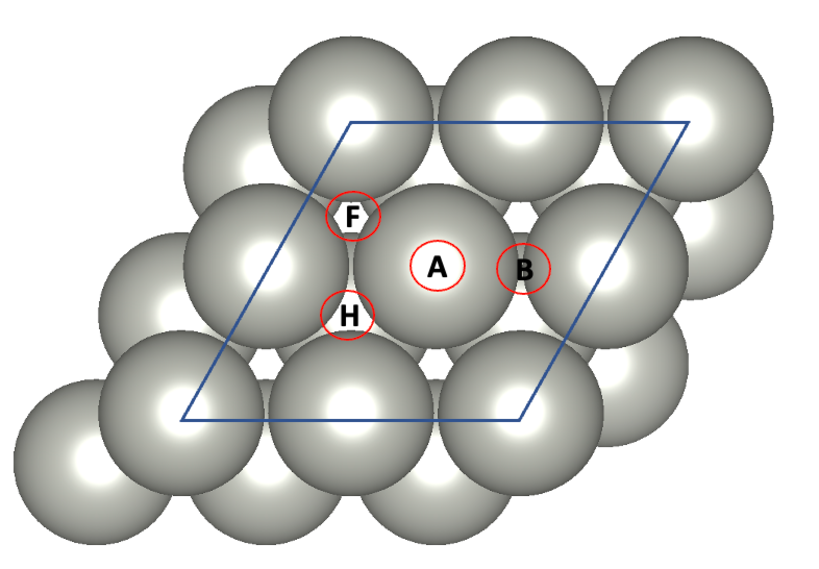
\includegraphics[width=10cm]{Figure/Pd.pdf}
	\caption{Geometric relationship between FCC, HCP, and Atop sites in the $(2 \times 2)$ supercell (blue lines) on the (111) surface of a close-packed metal. (F) , (H), (A) and (B) represent FCC, HCP,  Atop, and Bridge sites respectively.}
	\label{Pd}
\end{figure}

\subsection{Grand Canonical Monte Carlo (GCMC) Simulations} \label{GCMC_sec}
GCMC simulations were performed on the converged CE Hamiltonians with the Easy Monte Carlo Code (emc2) within ATAT \cite{VandeWalle2002}. The GCMC simulations provide information about coverage as a function of chemical potential ($\mu_{\ce{CO}}$), surface area $A$ and temperature $T$.  We performed GCMC simulations in a $42 \times 42$ supercell (1764 FCC Hollow sites, 1764 HCP Hollow sites, and 1764 Atop sites) from 100 K to 900 K and over a range of chemical potentials spanning coverages from 0 to $\approx 1$ CO/surface Pd. The calculations were initialized in a random configuration and the GCMC moves involve ``flipping'' a site between occupied and unoccupied states and were converged when the average coverage between steps $i$ to $j$ and $k$ to $l$ were within $10^{-5}$ ML of each other.

\section{Cluster Expansion Results}
\subsection{Comparison of CO Binding Sites}
To calibrate calculations, CO binding in FCC, HCP, atop and bridge sites were compared at $1/3$ ML in a $(\sqrt{3} \times \sqrt{3})R30^\mathrm{o}-1$ CO configuration (Table \ref{LowCOCoverage_table}). CO has similar  binding energies, vibrational frequencies and \ce{C-O} bond distances in the FCC and HCP sites, the bridge site is slightly less stable, and the atop site is the least stable by about $0.5$~eV over FCC/HCP. The generalized gradient approximation tends to exaggerate the preference of CO for high coordination sties \cite{Feibelman2001,Kresse2003}. However electron diffraction, vibrational spectroscopy and previous DFT calculations confirm the preference of CO for three-fold hollow sites at $1/3$ ML \cite{Lo1999, Ohtani1987, Fernandez1997}.

\begin{table} [t]
	\caption{Binding energies, \ce{C-O} bond lengths, and vibrational frequencies of CO at 1/3 ML in a $(\sqrt{3} \times \sqrt{3})R30^\mathrm{o}-1$ \ce{CO} Configuration}
	\footnotesize\setlength{\tabcolsep}{1pt}
	\centering
	\begin{tabular} {c c c c}
		\toprule
		Binding Site & Binding Energy & \ce{C-O} Bond Length (\AA) & Vibrational Frequency (cm$^{-1}$)\\
		\midrule
		FCC Hollow & $-2.00$ & 1.185 & 1820 \\
		HCP Hollow & $-2.01$ & 1.185 & 1822 \\
		Bridge     & $-1.81$ & 1.177 & 1878 \\
		Atop       & $-1.47$ & 1.156 & 2063 \\
		\bottomrule
	\end{tabular}
	\label{LowCOCoverage_table}
\end{table}

\subsection{Construction of Cluster Expansions}
\subsubsection{FCC-only Model}
We next considered coverage-dependent CO binding using a CE limited to the FCC sites as candidate coordination sites.  Table~\ref{CE_Cutoff_Radius} contains the details of the FCC-only CE fitting procedure.  We selected 25 seed structures from an initial candidate pool of 3164 possible structures and iterated the CE fitting procedure 3 times to arrive at a final, self-consistent CE.  The DFT database included at the end 58 structures, and the CE contains only one non-trivial two-body interaction (Table~\ref{fcc_ce}). 

\begin{table} [t]
	\caption{Summary Cluster Expansion Parameters}
	\centering
	\footnotesize\setlength{\tabcolsep}{2.5pt}
	\begin{tabular}{c c c c c}
		\toprule
		\multicolumn{2}{c}{CE Data} & FCC & FCC/HCP & FCC/HCP /Atop \\
		\midrule
		\multirow{3}{*}{Cluster Size (\AA)} & Pair     & 12.5 & 12.5 & 12.5\\
		& 3-Body   & 12.5 & 10.0 & 10.0\\
		& 4-Body   & 6.0  & 10.0 & 10.0\\
		\multicolumn{2}{c}{Structure Database} & 3164 & 6708 & 12280 \\
		\multicolumn{2}{c}{Cluster Database} & 131 & 870 & 1067 \\
		\multicolumn{2}{c}{Initial Number of Structures Included} & 25 & 63 & 50 \\
		\multicolumn{2}{c}{Iterations} & 3 & 21 & 6 \\
		\multicolumn{2}{c}{Final Number of Structures Included} & 58 & 183 & 193 \\
		\multicolumn{2}{c}{Clusters Included} & 3 & 47 & 43 \\
		\multicolumn{2}{c}{CV Score (meV/\AA$^2$)} & 7.59 & 9.62 & 9.08 \\
		\bottomrule
	\end{tabular}
	\label{CE_Cutoff_Radius}
\end{table}

 Figure \ref{AllCE} C compares the GGA-computed formation energies with the CE predictions.  The two-body-only CE fits the data with a cross validation score of 7.59 meV/\AA$^2$. Figure \ref{AllCE} A shows the DFT-computed formation energies.  The minimum energy hull has two ``kinks''  at $1/3$ and $2/3$ ML corresponding to a $(\sqrt{3} \times \sqrt{3})R30^\mathrm{o}-1$ \ce{CO}  (Figure \ref{GroundStates} A) and a $(\sqrt{3} \times \sqrt{3})R30^\mathrm{o}-2$ \ce{CO} configuration (Figure \ref{GroundStates} B), respectively.  Figure \ref{GroundStates} C includes for completeness the  $(1 \times 1)$ structure.  The slope of the formation energy hull is the 0~K  differential binding energy, $\bar{E}_{\ce{CO}}^{\text{FCC}}(\theta,0~\text{K})$, and is plotted in  Figure \ref{AllCE}  B.  The 0 K differential binding energy is constant to $1/3$~ML, up to which coverage each adsorbate can avoid any first nearest neighbor (1NN) interactions, steps up above $1/3$ ML as each new adsorbate accumulates three 1NNs, and steps up again to a positive value above $2/3$~ML, where each new adsorbate acquires 6 1NNs. Table \ref{OneSiteGroundStatesTable} summarizes the ground state geometries in this model and Supplementary Section \ref{fccCE} provides the CE details. 

\begin{figure} [ht]
	\centering
	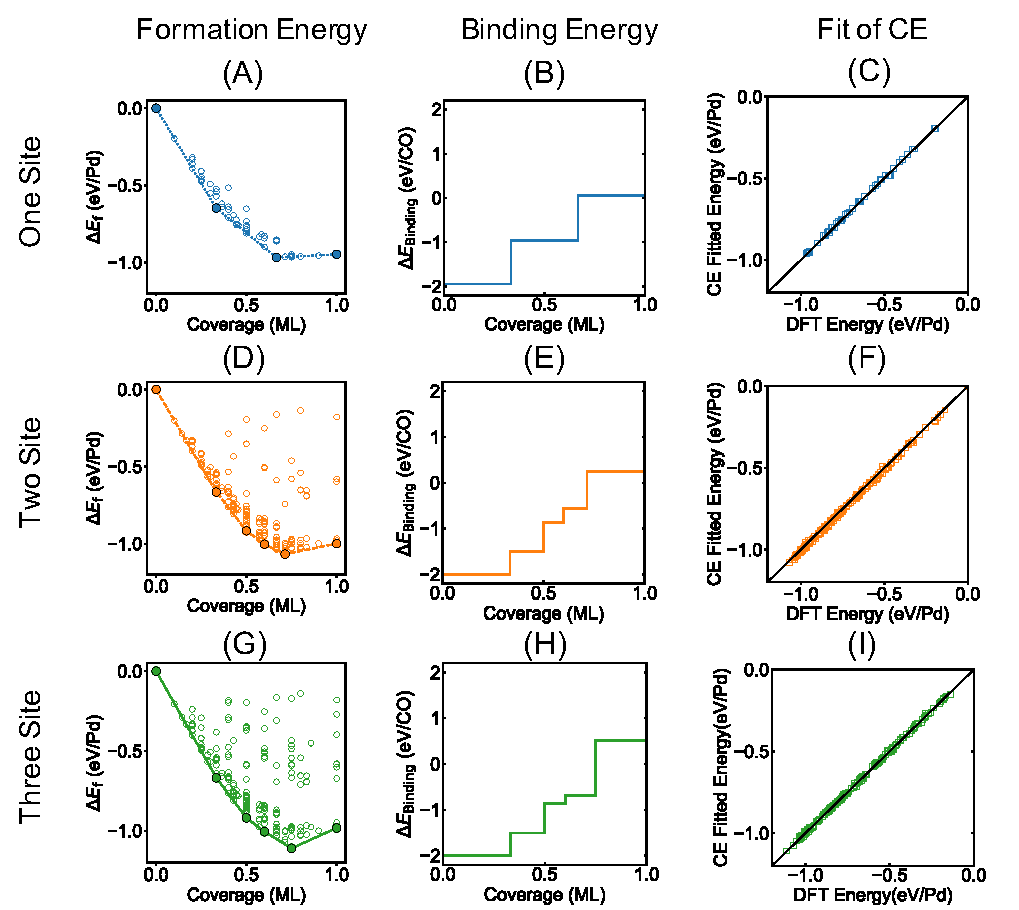
\includegraphics[width=15cm]{Figure/AllCE.pdf}
	\caption{
		First column: GGA-computed formation energies vs.\ coverage for FCC-only, FCC/HCP, and FCC/HCP/atop models from top to bottom. Middle column: differential binding energy vs.\ coverage for same three models. Last column: CE fitted vs.\ DFT-computed formation energies for same three models.}  
	\label{AllCE}
\end{figure}
\clearpage

\begin{figure} [ht]
	\centering
	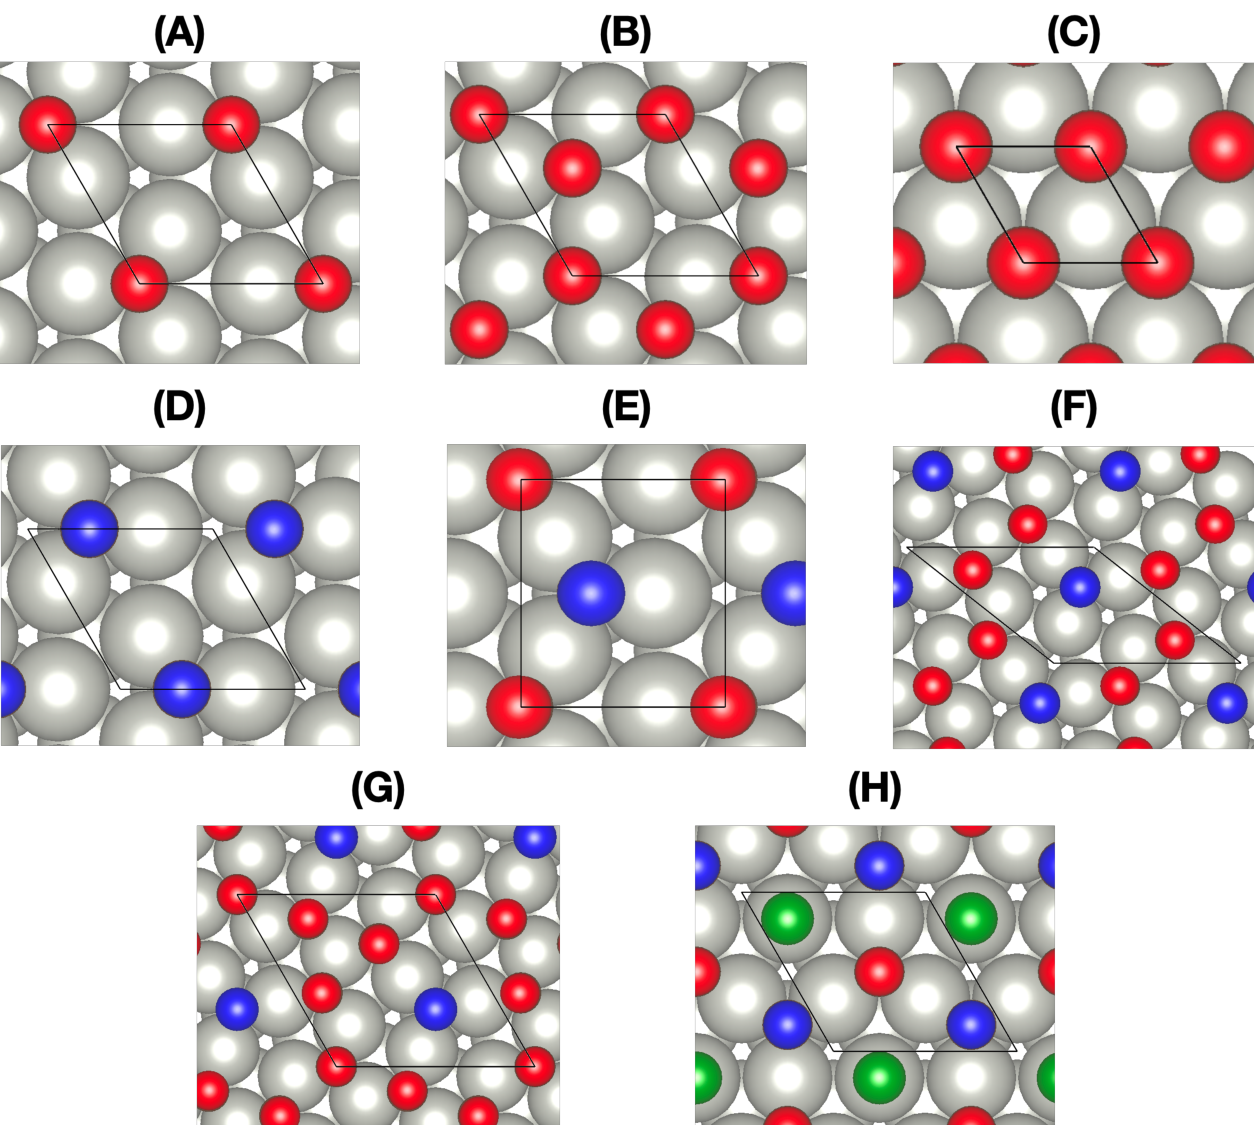
\includegraphics[width=0.9\textwidth]{Figure/Gs1.pdf}
	\caption{Top view of computed ground state structures.  Red, blue and green correspond to FCC, HCP, and atop sites, respectively.  (A) 1/3 ML FCC, (B) 2/3 ML FCC, (C) 1 ML FCC, (D) $1/3$ ML HCP Hollow, (E) $1/2$ ML FCC/HCP, (F) $3/5$ ML FCC/HCP, (G) $5/7$ ML FCC/HCP, and (H) $3/4$ ML FCC/HCP/ATOP. Black lines represent the unit cell.}
	\label{GroundStates}
\end{figure}

\begin{table} [t]
	\caption{Geometric Data for the FCC Hollow Site Cluster Expansion Ground States.} 
	\centering
	\begin{tabular} {c c}
		\toprule
		Coverage (ML) & Geometry\\
		\midrule
		1/3                      & $(\sqrt{3}\times\sqrt{3})R30^\mathrm{o}-1$ \ce{CO} \\
		\\
		2/3     & $(\sqrt{3}\times\sqrt{3})R30^\mathrm{o}-2$ \ce{CO} \\
		\\
		1                        & ($1\times1$)-1 \ce{CO} \\
		\bottomrule
	\end{tabular}
	\label{OneSiteGroundStatesTable}
\end{table}

\subsubsection{FCC/HCP Model}
We next considered CO co-adsorption in FCC and HCP sites.  In principle, these two sublattices together can accommodate up to two CO molecules per surface Pd atom.  Adjacent FCC and HCP sites are separated by only 1.615~\AA, and test calculations show that two CO placed this close to one another relax spontaneously to more remote sites.  We estimate this 1NN FCC-HCP interaction energy to be approximately 2~eV, greater than the absolute CO binding energy at low coverage.   
Above a coverage of 1 CO molecule per surface Pd these 1NN FCC-HCP interactions are unavoidable.  Further tests show that at these high coverages, CO molecules near the surface relax to unphysical structures in which the \ce{C-O} bond is broken. Thus, we found it necessary to exclude all FCC/HCP structures with a total coverage $> 1$~ML and, to obtain energies useful for inclusion in the DFT database, to laterally constrain CO pairs in 1NN FCC-HCP adjacency in configurations below 1~ML.  

Table \ref{CE_Cutoff_Radius} contains the results of the cluster expansion fitting procedure. We initially selected 63 structures from a candidate pool of 6708, including all the structures from the FCC-only calculations and additional HCP-only and mixed configurations. The fitting procedure took 21 cycles to converge to a self-consistent CE.  A total of 183 DFT structures were computed, and the final CE including 47 clusters had a CV score of 9.62 meV \AA$^{-2}$ (Table~\ref{fcchcp_ce}). Figure \ref{AllCE} F shows that the CE reproduces the DFT numbers uniformly well.  The inclusion of FCC and HCP sites together yields a richer formation energy hull, shown in Figure \ref{AllCE} D. The ground state at $1/3$~ML remains and has the same $(\sqrt{3} \times \sqrt{3})R30^\circ-1$ \ce{CO} structure, although as expected from the comparisons in Table~\ref{LowCOCoverage_table}, with CO in HCP sites (Figure \ref{GroundStates} D).  A new ground state appears at $1/2$ ML in which half the CO occupy FCC and half HCP sites, each CO sublattice having c$(4\times2)$ symmetry (Figure \ref{GroundStates} E).  In this configuration half the surface Pd have two CO in opposing (second nearest neighbor, 2NN) FCC and HCP sites and the other half have either a single FCC or HCP CO.  Another new ground state appears at $3/5$ ML (Figure \ref{GroundStates} F) in which $2/3$ of the CO occupy FCC and $1/3$ HCP sites.  Here the FCC CO form chains of adjacent occupied sites like that in the $2/3$ ML FCC-only structure, with the chains separated by intervening rows of HCP CO.  The more dense $2/3$ ML FCC-only ground state disappears in the FCC/HCP system.  In its place appears a $5/7$ ML structure (Figure~\ref{GroundStates} G) in which $4/5$ of the CO occupy FCC and $1/5$ HCP sites.  The structure is more complex, but the 2NN FCC-HCP motif is retained.  At $1$ ML the FCC-only configuration is lower in energy than HCP-only; any mixed configuration would have high energy 1NN CO. As evident from Figure \ref{AllCE} D, many other configurations are close in energy to the ground state hull.  Figure \ref{AllCE} E plots the differential binding energy $\bar{E}_{\ce{CO}}^{\mathrm{F/H}}(\theta)$ extracted from the ground state hull.  Energies increase in more gradual steps than in the FCC-only model up to $5/7$ ML, where $\bar{E}_{\ce{CO}}^{\text{F/H}}(\theta)$ jumps to a strongly positive value.  Table \ref{twositegstable} summaries the structures for the ground states and Supplemental Section~\ref{FCCHCPSiteCE} contains details of the FCC/HCP CE. 

\begin{table} [t]
	\caption{Geometric Data for the FCC and HCP Hollow Site Cluster Expansion Ground States.}
	\centering
	\begin{tabular} {c c}
		\toprule
		Coverage (ML) & Geometry\\
		\midrule
		1/3                   &  ($\sqrt{3}\times\sqrt{3})R30^\mathrm{o}-1$ \ce{CO} \\
		\\
		1/2  & c$(4\times2)-$2 \ce{CO}             \\
		\\
		3/5  & $|a|=|b|=7.399$ \AA, $\psi$=141.78$^\mathrm{o}$ \\
		\\
		5/7  & $|a|=|b|=7.399$ \AA, $\psi$=120.00$^\mathrm{o}$\\
		\\
		1                     &  ($1\times1)-$1 \ce{CO} \\
		\bottomrule
	\end{tabular}
	\label{twositegstable}
\end{table}

\subsubsection{FCC/HCP/Atop Model} 

We next consider CO adsorption into FCC, HCP, and atop sites (Figure \ref{Pd}). In principle, these three sublattices can accommodate up to three CO per surface Pd atom. First-nearest-neighbor separations between any pair of sublattices is 1.615~\AA. Test calculations report results similar results to those above; any 1NN pairing is of very high energy, unstable, and unimportant.  Again we prune from the DFT database all structures with $> 1$~ML coverage and constrain the positions of 1NN pairs to preserve site occupances at $< 1$~ML.Table \ref{CE_Cutoff_Radius} contains the results of the converged cluster expansion.  The candidate pool includes 12280 candidate DFT structures, which included all of the strucutres from the previous models, plus atop-only and mixed (FCC/HCP/atop) configurations.  We started with 50 initial structures, chosen at random. The CE fitting procedure converges after 6 iterations and the computation of a total of 193 DFT structures.  

Fitting only requires ten more DFT energies and four fewer clusters to obtain a cross validation score of 9.08 meV/\AA$^2$. Figure \ref{AllCE} I shows a comparison of the DFT computed formation energies with the cluster expansion predicted formation energies. Figure \ref{AllCE} G shows the DFT formation energies with the formation energy hull, where there are ``kinks'' at $1/3$, $1/2$, $3/5$, and $3/4$ ML, which correspond to the ground states. The ground states at $1/3$, $1/2$, $3/5$ and $1$ ML are the same ground states determined in by the FCC, and HCP Hollow site cluster expansion (Figure \ref{GroundStates} C-F). A new ground state at $3/4$ ML has CO adsorbed in a FCC Hollow, HCP Hollow and Atop site. Figure \ref{AllCE} H shows the 0 K differential binding energy, where there are steps at 0, $1/3$, $1/2$, $3/5$, and $3/4$ ML. At $3/4$ ML, the 0 K differential binding energy becomes positive, which is different from the previous models. 

Table \ref{threesitegstable} reports the geometric configurations for the ground states, and Section \ref{FCCHCPAtopSiteCE} in the Supplemental Information contains all of the effective cluster interactions, and clusters included in the converged cluster expansion. Figure~\ref{DFTcompare} in the Supplementary Information shows a comparison of the formation energies for the different models, and Figure~\ref{DiffBindingEnergy} in the Supplemental Information shows a comparison of the differential binding energies for the different models

\begin{table} [t]
	\caption{Geometric Data for the FCC, HCP Hollow, and Atop Site Cluster Expansion Ground States.}
	\centering
	\begin{tabular} {c c}
		\toprule
		Coverage (ML) & Geometry\\
		\midrule
		1/3   &  ($\sqrt{3}\times\sqrt{3})R30^\mathrm{o}-1$ \ce{CO} \\
		\\
		1/2  & c$(4\times2)-$2 \ce{CO}             \\
		\\
		3/5  & $|a|=|b|=7.399$ \AA, $\psi$=141.78$^\mathrm{o}$ \\
		\\
		3/4  & $(2\times2)-3$ \ce{CO}\\
		\\
		1                     &  ($1\times1)-$1 \ce{CO} \\
		\bottomrule
	\end{tabular}
	\label{threesitegstable}
\end{table}

\subsection{Comparison to Previous Work}

The full cluster expansion construction procedure successfully recovers the known ground states of CO on Pd(111).  In particular, the three most prominent ground states, as judged by the magnitude of the discontinuities in the coverage-dependent binding energy (Figure \ref{AllCE} H), including the HCP-only configuration at $1/3$ ML, the mixed FCC/HCP configuration at $1/2$ ML, and the FCC/HCP/Atop configuration at $3/4$ ML, all correspond with configurations observed by electron diffraction \cite{Ohtani1987, Surnev2000, Schaff1998} and infrared spectroscopy \cite{Bradshaw1978, Hoffmann1983} as well as DFT \cite{Lo1999, Martin2014, Rose2002}.  The CE predicts a more minor ground state at $3/5$ ML that to our knowledge has not been observed. 

Chen \cite{Chen2012} recently reported a cluster expansion for CO on Pd(111).  The CE included FCC, HCP, Atop, and bridge sites, was fitted against 94 pre-selected configurations computed using the RPBE functional, and included only two-body interaction terms. The RPBE functional produces an approximately constant offset of 0.2 eV/CO in binding energy relatively to the PW91 functional used here.\cite{Herron2012}  The qualitative features of the predicted hull are similar to those found here, although the Chen CE contains a larger number of ground states and saturation at a somewhat lower coverage. 

\section{Coverage-Dependent Binding Energies}

It is common to introduce a coverage-dependent (partial molar) binding energy, $\bar{E}(\theta)$, in mean-field kinetic models. There is however no generally accepted strategy for obtaining the binding energy from first-principles \cite{Grabow2008, Gokhale2008, Stamatakis2011a, Stamatakis2011, Getman2010, Park1999, Aghalayam2003, Hansgen2010, Aghalayam2000}. A coverage-dependent CO binding energy is necessary to recover WGS kinetics over Pd, Pt and Cu and is often obtained by DFT calculations on a small number of arbitrary adsorbate coverages and configurations \cite{Grabow2008, Gokhale2008, Stamatakis2011a, Stamatakis2011}. As is evident from the 0~K differential binding energies shown in the middle column of Figure \ref{AllCE} and Supplementary Figure~\ref{DiffBindingEnergy}, the differential binding energies at the coverages that are relevant to WGS are sensitive to these choices.  As is also evident, differentiation of the 0~K energy hull produces discontinuities in coverage-dependent properties that are inappropriate to include in $\bar{E}(\theta)$.  Here we extract $\bar{E}(\theta)$ from finite-temperature Monte Carlo simulations.

\subsection{Determination of \texorpdfstring{$\bar{E}(\theta)$}{lg} by GCMC}

Grand canonical Monte Carlo (GCMC) simulations on the cluster expansion Hamiltonian at temperature $T$ gives the coverage ($\theta$) versus the chemical potential ($\mu_{\ce{CO}}$). The chemical potential is related to the binding energy by:

\begin{equation} \label{GCMC_mu_eq}
	\mu_{\ce{CO}}(\theta,T) = \bar{E}_{\ce{CO}}(\theta,T) - T \bar{S}_{\ce{CO}}(\theta,T)
\end{equation}

\noindent where $\bar{E}_{\ce{CO}}(\theta,T)$ and $\bar{S}_{\ce{CO}}(\theta,T)$ are the partial molar enthalpy and entropy, respectively. Within a single-site mean field model, and considering only configurational entropy,  $\bar{S}_{\text{MF}}(\theta,T)$ is given by:\cite{Baker1966, Fowler1936}

\begin{equation} \label{entropy_one_meanfield}
	\bar{S}_\text{MF}(\theta,T) = -k_B T \ln \left ( \frac{\theta}{1-\theta} \right )
\end{equation}

\noindent which generalizes to $n$-sites as

\begin{equation} \label{entropy_n_meanfield}
	\bar{S}_\text{MF}(\theta,T) = -k_B T \ln \left ( \frac{\theta}{n*(1-\theta)} \right )
\end{equation}

\noindent as derived in Supplementary Section~\ref{entropytreatment}. An effective mean-field coverage-dependent binding energy can then be defined as 

\begin{equation} \label{ECO}
	\bar{E}_{\ce{CO}}(\theta,T) = \mu_{\ce{CO}}(\theta,T) + T\bar{S}_{\text{MF}}(\theta,T)
\end{equation}

\subsection{GCMC Results}

\begin{figure} [h]
\centering
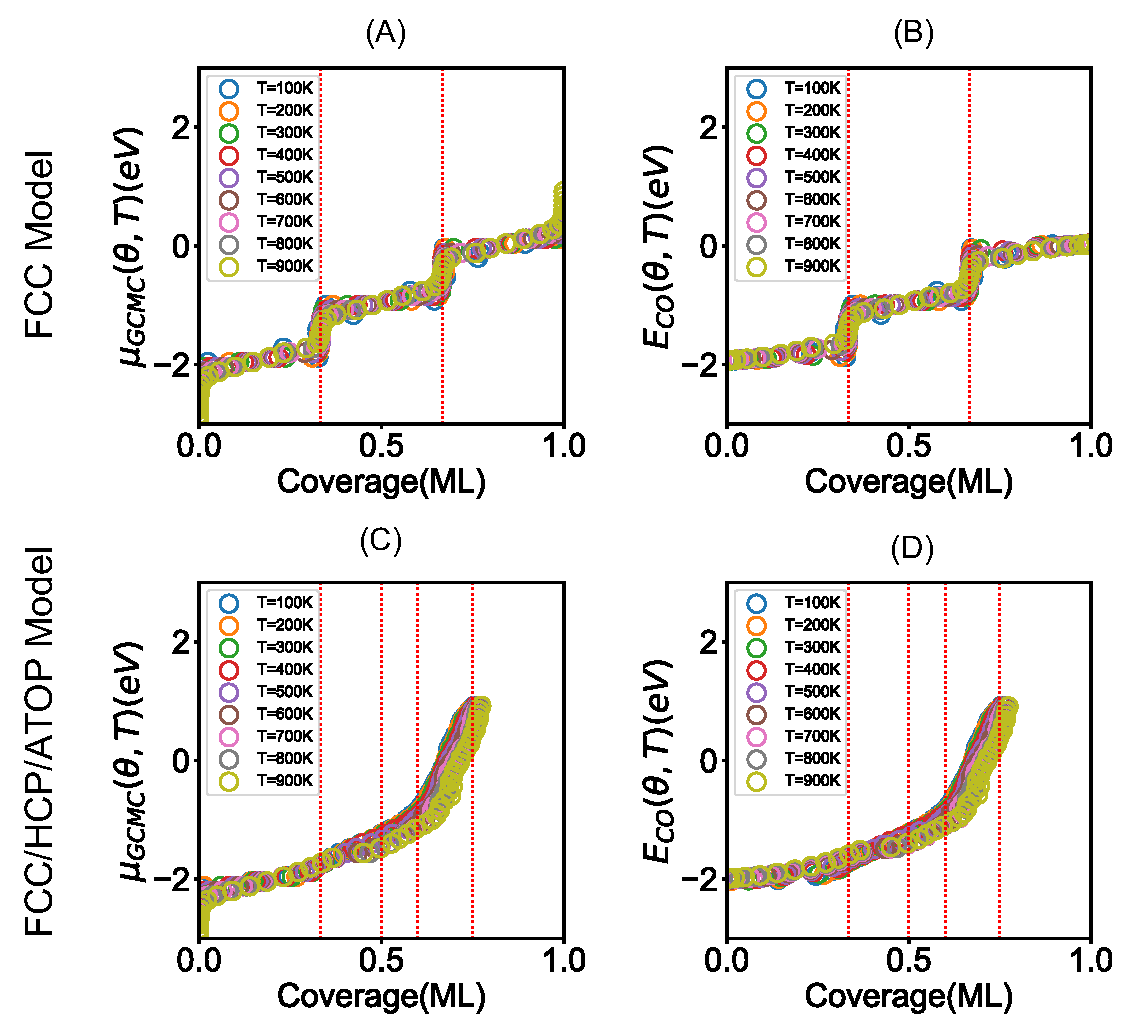
\includegraphics[width=15cm]{Figure/GCMC1.pdf}
\caption{First column: $\mu_{\ce{CO}}(\theta,T)$ vs.\ coverage for FCC model and FCC/HCP/ATOP models from top to bottom at temperature range from 100K to 900K. Last column: $E_{\ce{CO}}(\theta,T)$ vs.\ coverage for the same models.}
\label{sumgcmc}
\end{figure}

\noindent
GCMC simulations were performed from 100K to 900K on the one-site and three-site CE models. Each temperature perform five times and then take average value. Results are shown in Figure \ref{sumgcmc} A and C, plotted as $\mu_{\ce{GCMC}}(\theta,T)$ vs.\ $\theta_{\text{CO}}$. 
In Figure \ref{sumgcmc} A, the chemical potential diverges in the limits of 0 and 1~ML, reflecting the divergence of Eq.~\ref{GCMC_mu_eq} in those limits. In Figure \ref{sumgcmc} C, the chemical potential diverges in the limits of 0 ML.
The one-site model (Figure~\ref{sumgcmc} A) retains the 0~K stair-step pattern smeared out at the boundaries of each ground states. The three site model (Figure~\ref{sumgcmc} C) shows a qualitatively different gradual rise in chemical potential to approximately 0.6~ML, followed by a sharper rise from 0.6 to 0.75 ML.
Figure \ref{sumgcmc} B and D shows $\bar{E}_{\ce{CO}}(\theta,T)$ vs.\ $\theta$ extracted using Eq~\ref{ECO}. Subtraction of the mean-field configurational entropy eliminates the divergences at the extremes of coverage and damps the rise in energy at intermediate coverage. Further, the sharp discontinuities present in the 0~K differential binding energies are smeared out at finite temperature. Figure \ref{sumgcmc} B and D show that the differential binding energies extracted this way are only weakly temperature dependent. 

\subsection{Coverage-Dependent Binding Energy Models}\label{co-model}

For the purposes of microkinetic modeling it is convenient to represent $\bar{E}(\theta)$ in analytical form.  Piece-wise linear \cite{Grabow2010}, activity \cite{Bajpai2020} and logistic\cite{Grabow2008} forms have all been applied to obtain analytical binding energy expression. Here, we fit the one-site and three-site binding energies to the following analytic functions:

\begin{align*}
\text{Piece-wise linear:} & \quad \overline{E}_{\ce{CO}}(\theta) = A \text{ for }\theta<C\text{  and }A+B(\theta-C)\text{ for } \theta\geq C\\
\text{Activity:} & \quad \overline{E}_{\ce{CO}}(\theta)  =A+B\left\{\frac{\lambda_{1}}{1+\lambda_{1}\theta}+\ln\left(\frac{1+\lambda_{2}\theta}{1+\lambda_{1}\theta}\right)+\theta\left[\frac{\lambda_{2}-\lambda_{1}}{(1+\lambda_{2}\theta)(1+\lambda_{1}\theta)}\right]\right\}\\
\text{Logistic:} & \quad \overline{E}_{\ce{CO}}(\theta)  =\frac{A}{1+ \exp (B(\theta_{\text{CO}}- C ))}+D\\
\end{align*}

\noindent
For piecewise function, the data divided to several part by using scipy.optimize with Python. Then implement polyfit to obtain piecewise function. For logistic and activity function, curve\_fit is employed from scipy.optimize package to perform fitting with data. Figure \ref{fit13} plots the fitted binding energies against the GCMC-inferred binding energies. Results are summarized in Table \ref{sumfit}. Not surprisingly, only Piecewise model is sufficiently flexible to capture the stair-step pattern of the the FCC-only model (Figure~\ref{fit13} A) with mean absolute error are as small as 0.0397 eV/CO. But Logistic and Activity model are not able to capture stair-up feature with mean absolute errors are as large as 0.106 and 0.145 eV/CO. The fits keep fluctuating with coverage increase and the estimation of binding energy are far from precision. \par
For the three-site model, all of the fits show the same trend in that at low coverages (high negative bonding energies), the fits correctly estimate the binding energy. At moderate coverages, the fits fluctuate between over and under estimating the binding energies. At high coverages, the all of the fits approriately estimate the binding energies (Figure \ref{fit13} D-F). For the three site model fitting up to a coverage $\theta\approx$ 0.75 ML, the largest mean absolute error is 0.126~eV/CO for the Logistic and Activity fit. For determination of the best fit, the Piecewise functions had the highest R$^2$ value and the lowest mean absolute error across all the different models studied for both the one-site and three-site binding energy models.

\begin{figure} [h]
\centering
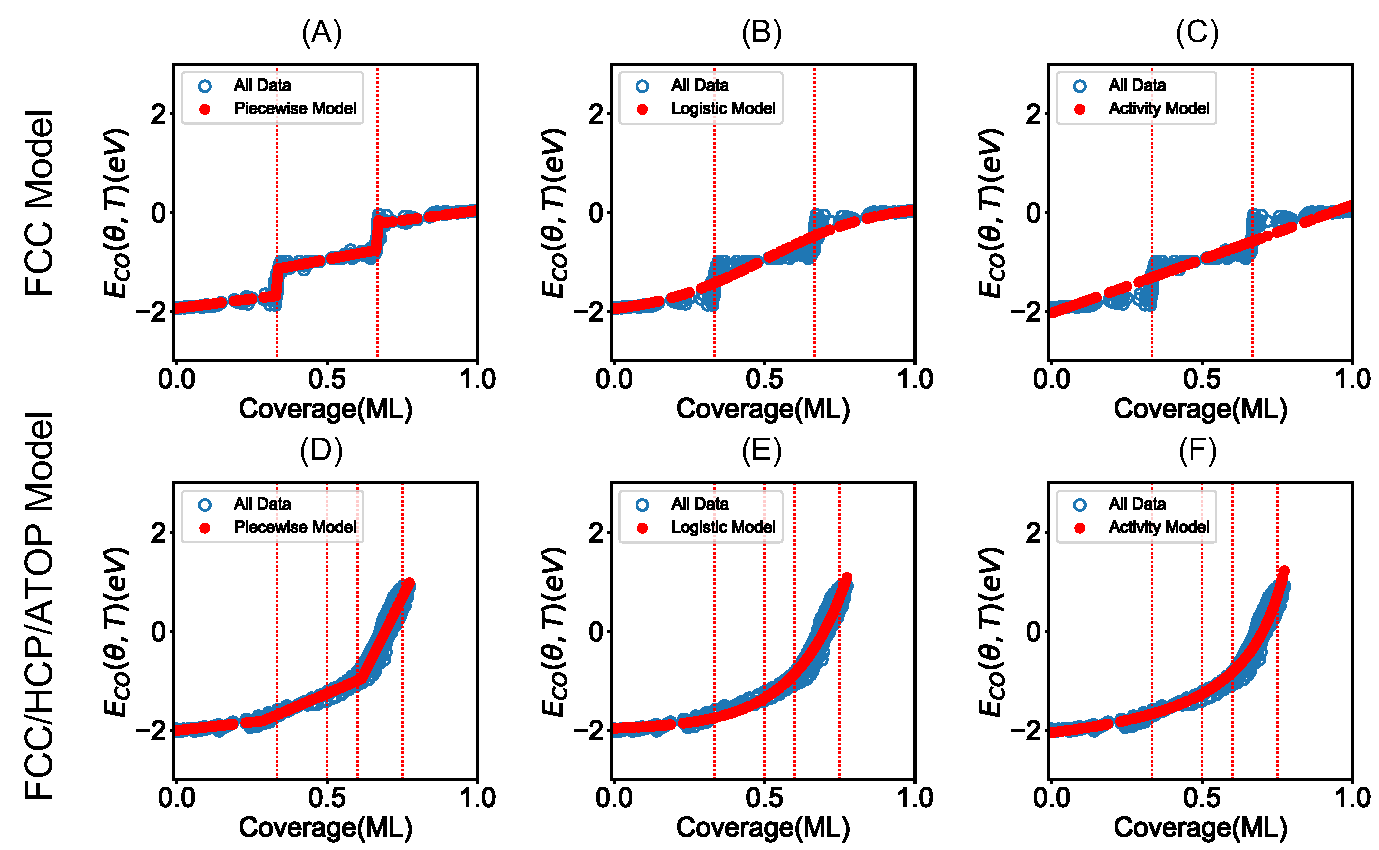
\includegraphics[width=15cm]{Figure/fitting13.pdf}
\caption{First column: piecewise model fit to all data point. Second column: logistic model fit to all data point. Third column: activity model fit to all data point.}
\label{fit13}
\end{figure}

\begin{table} [h]
\caption{Analytical Fitting Result for FCC Model and FCC/HCP/Atop Model }
\centering
\setlength{\tabcolsep}{6pt}
\renewcommand{\arraystretch}{1.5}
\begin{tabular} {c c c c c c c}
\toprule
 & & FCC Model& & & FCC/HCP/Atop Model\\
%\midrule
\cmidrule[\heavyrulewidth](lr){2-4}\cmidrule[\heavyrulewidth](lr){5-7}
Function & R$^2$&MAE&MSE& R$^2$&MAE&MSE\\
\midrule
Piecewise   &0.977 &0.0397&0.00391&0.975&0.110&0.00224\\
\\
Logistic  & 0.958 &0.106&0.0218&0.97&0.126&0.0265\\
\\
Activity  & 0.938 &0.145&0.0323&0.968&0.126&0.0285 \\
\bottomrule
\end{tabular}
\label{sumfit}
\end{table}

\clearpage
\subsection{Temperature Programmed Desorption (TPD)}

The CO TPD spectrum on Pd(111) (Figure \ref{Exp_TPD}) has been thoroughly studied by Guo and Yates, and the shape of the TPD reflects the coverage dependent binding energies \cite{Guo1989}. In this work a simulated TPD was generated using the GCMC results for the coverage-dependent binding energy and all of the analytical fits for coverage dependent binding energy and the first-order Polyani-Wigner Equation (equation \ref{redhead}), where $\beta$ is the heating rate (2 K$/$s), and $\nu$ is the prefactor (10$^{13}$ s$^{-1}$, independent of coverage) \cite{Redhead1962}. The synthetic TPD can be determined by numerical integration in steps of 0.2 K starting from 100 K to 800 K and initial coverages varying from 0.1 to 0.6 ML.

\begin{equation} \label{redhead}
	r_\mathrm{Des}=-\frac{\partial \theta}{\partial T}=\frac{\nu \theta}{\beta} \exp \left( - \frac{\overline{E}_\mathrm{CO}(\theta)}{k_\mathrm{B} T} \right)
\end{equation}

\begin{figure} [ht]
	\centering
	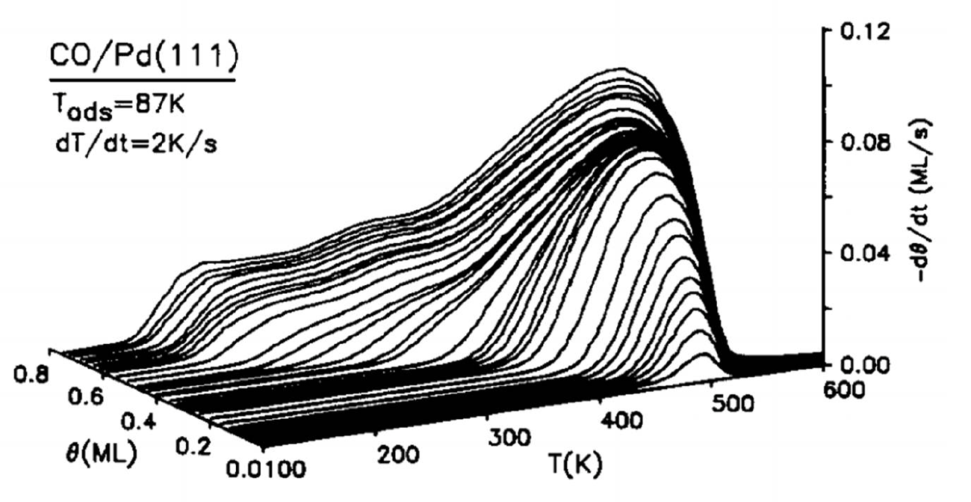
\includegraphics[width=0.9\textwidth]{Figure/Ex_TPD.pdf}
	\caption{Experimental TPD obtained by Guo and Yates. Heating Rate is 2 K/s, and CO was adsorbed at 87 K. Taken from Reference \cite{Guo1989}.}
	\label{Exp_TPD}
\end{figure}

The simulated TPD spectrum are shown in Figure \ref{tpd}.  Figure \ref{tpd} A-C are TPD spectrum with different analytical fits of FCC model. As initial coverage up to 0.3 ML, Figure \ref{tpd} A give a single peak around 680 K, approximately 180 K higher than the experimental peak which is due to GGA function tend to overestimate binding strength of CO on Pd \cite{Perdew1996, Herron2012,wellendorff2015}.As the initial coverage increases above 0.4 ML, a second sharp peak appears around 350 K. And when initial coverage keep increasing, the second peak shift to lower temperature. In Figure \ref{tpd} B, when initial coverage up to 0.3 ML, single peak occur around 680K but the intensity are same for 0.2 and 0.3 ML. As initial coverage increase to 0.6 ML, second peak shows up around 250K which is absent in the experimental TPD. In Figure \ref{tpd} C, as initial coverage increase, the overall TPD trend are also increasing which is totally opposite to experimental TPD. Based on the TPD plot, it suggests that single site model cannot reflect actual coverage-dependent binding energy and TPD spectra varies also depend on the analytical model chosen.

Figure \ref{tpd} D-F are TPD spectrum with different analytical fits of FCC/HCP/Atop model. As initial coverage up to 0.3 ML, Figure \ref{tpd} D give a peak around 680K and peak shift slightly. When coverage increase to 0.4 ML, the TPD occur a polyline around 600K, and the reason is that piecewise function has an intersection point about 0.3 ML and the derivative is not continuous at that point so TPD has a turning point when initial coverage above 0.3 ML. Figure \ref{tpd} E and F has the general shape that is more consistent with the experimental TPD. A low coverage peak occurs around 680 K, and grows until an initial coverage of 0.3 ML. The longer leading edge at higher coverages arises from the more gradual variation in the coverage-dependent binding energy. Although the shape of TPD spectra are different, the peak temperature stay constant within logistic and activity model. 
 In section \ref{co-model}, fitting results show that piecewise function has the best fit result, but based on Figure \ref{tpd} D-F, logistic function perform better in simulating TPD spectra.


\begin{figure}[t]
	\centering
	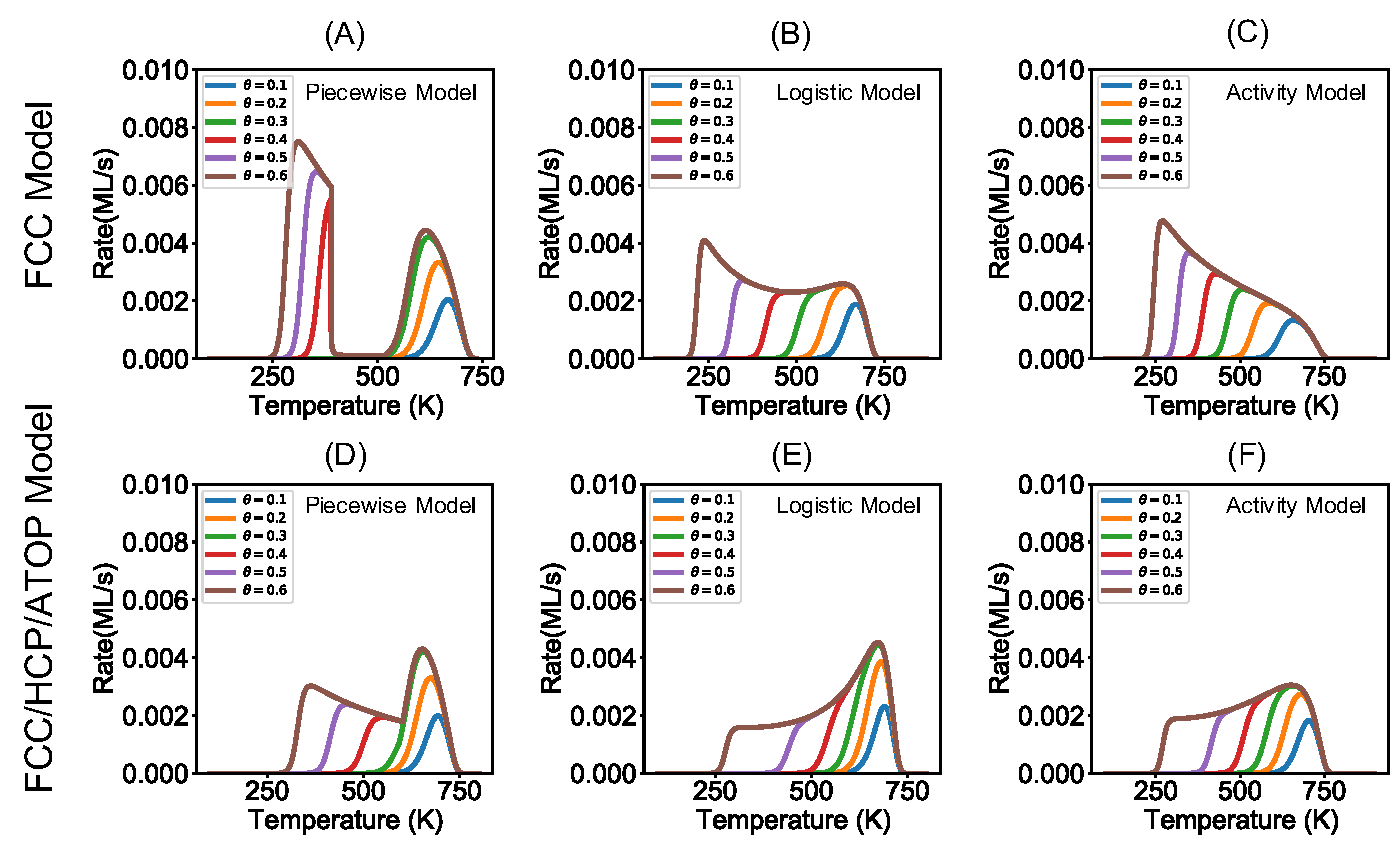
\includegraphics[width=\textwidth]{Figure/tpd13.pdf}
	\caption{TPD Spectrum for the One and Three Site Model. (A) FCC Hollow Site Model, desorption rate is proportional to $\theta$, (B) FCC, HCP Hollow, and Atop Site Model, desorption rate is proportional to $\theta$}
	\label{tpd}
\end{figure}

\clearpage
\section{Conclusions}
A cluster expansion is a useful approach for exploring the coverage-dependent binding in multi-site systems, such as CO on Pd(111). For CO adsorbed on Pd(111), inclusion of multiple sites in CE is necessary to properly capture the coverage-dependent binding behavior. Using the cluster expansion, GCMC simulations were used to extract the coverage-dependent binding energy appropriately for mean-field models. Three analytical functions are used to fit coverage-dependent binding energy for simulating TPD spectra. Three site model TPD can recover general shape and high temperature peak compare to experimental result which indicate that combination of cluster expansion and GCMC simulation can accurately capture coverage-dependent binding energy of CO on Pd. \\

\pdfbookmark[1]{Acknowledgment}{Acknowledgment}
\textbf{Acknowledgment} This work was supported by the US Department of Energy Chemical Sciences Program grant number DE-FG02-03ER15466. Computational support was provided by the Notre Dame Center for Research Computing.

\clearpage
\printbibliography

\clearpage
\section*{Supplemental Information}
\makeatletter
\renewcommand{\thetable}{S\@arabic\c@table}
\renewcommand{\thefigure}{S\@arabic\c@figure}
\renewcommand{\thesection}{S\@arabic\c@section}
\renewcommand{\theequation}{S\@arabic\c@equation}
\makeatother

\setcounter{section}{0}
\setcounter{table}{0}
\setcounter{figure}{0}
\setcounter{equation}{0}

\section{FCC Hollow Site Cluster Expansion} \label{fccCE}
The lat.in file sets up the CE and the adsorption sites. The file is used create the structure database and cluster database. The first line of the file sets up the unit cell. Lines 2-5 are the unit cell vectors. The remaining lines set specify the atom positions and types.

The lat.in file for the FCC Hollow Site model is:
\begin{verbatim}
2.79658 2.79658 27.9658 90 90 60
1 0 0
0 1 0
0 0 1
0.0000000000000000 0.0000000000000000 0.0000000000000000 Pd_F
0.3333333333333333 0.3333333333333333 0.0817570000000032 Pd_F
0.6666666666666666 0.6666666666666666 0.1672046730538995 Pd_T
0.0000000000000000 0.0000000000000000 0.2168483413880288 Vac,CO_T
\end{verbatim}

%\clearpage
\begin{table} [ht]
\caption{Clusters Included in the Final FCC Hollow Site Cluster Expansion and Corresponding Interacting Coefficients.  Cluster refers to the cluster number in the clusters.out file. Type refers to the number of sites in the cluster (1-body, 2-body, etc). ECIMULT is the ECI times the multiplicity and then converted from a per site basis to a per atom basis, and is used by ATAT.} %\red{What is Cluster?  Type? ECIMULT?  Is this sufficient information for someone else to recreate this CE?} } 
\centering
\begin{tabular} {c c c c c c}
\toprule
Cluster & Type & Radius (\AA)& Multiplicity & ECI ($\frac{\mathrm{eV}}{\mathrm{site}}$) & ECIMULT ($\frac{\mathrm{eV}}{\mathrm{atom}}$) \\
\midrule
1 &	0 &	0.0000	& 1 &	-15.226	  &      -3.80649 \\
2 &	1 &	0.0000  & 1 &	-0.47508  &	-0.11877  \\
3 &	2 &	2.79658	& 3 &	0.0816056 &	0.0612042 \\
\bottomrule
\end{tabular}
\label{fcc_ce}
\end{table}

The clusters.out file contains all of the possible clusters that can be used in the fit. For each cluster, each line has the following meaning:
\begin{verbatim}
Multiplicity
Radius
Number of Points in Cluster
[Coordinates of 1st point] [Number of possible species] [Cluster Function]
[Coordinates of 2st point] [Number of possible species] [Cluster Function]
\end{verbatim}

For the FCC Hollow Site model the clusters included are (each cluster separated by a blank line):
\begin{verbatim}
1
0.00000
0

1
0.00000
1
1.00000     1.00000     0.21685 0 0

3
2.79658
2
1.00000      1.00000    0.21685 0 0
1.00000     -0.00000    0.21685 0 0
\end{verbatim}

\clearpage
\section{FCC, and HCP Hollow Site Model} \label{FCCHCPSiteCE}

The lat.in file for the FCC, HCP Hollow Site model is:
\begin{verbatim}
2.79658 2.79658 27.9658 90 90 60
1 0 0
0 1 0
0 0 1
0.0000000000000000 0.0000000000000000 0.0000000000000000 Pd_F
0.3333333333333333 0.3333333333333333 0.0817570000000032 Pd_F
0.6666666666666666 0.6666666666666666 0.1672046730538995 Pd_T
0.0000000000000000 0.0000000000000000 0.2168483413880288 Vac,CO_T
0.3333333333333333 0.3333333333333333 0.2168483413880288 Vac,CO_T
\end{verbatim}

%\clearpage
\begin{longtable} {c c c c c c}
\caption{Clusters Included in the Final FCC, and HCP Hollow Site Cluster Expansion and Corresponding Interaction Coefficients. Cluster refers to the cluster number in the clusters.out file. Type refers to the number of sites in the cluster (1-body, 2-body, etc). ECIMULT is the ECI times the multiplicity and then converted from a per site basis to a per atom basis, and is used by ATAT.} \label{fcchcp_ce} \\
\toprule
 Cluster & Type & Radius (\AA) & Multiplicity & ECI ($\frac{\mathrm{eV}}{\mathrm{site}}$) & ECIMULT ($\frac{\mathrm{eV}}{\mathrm{atom}}$) \\
\midrule \endfirsthead

\caption[]{{\em Continued}}\\
\midrule
Cluster & Type & Radius (\AA)& Multiplicity & ECI ($\frac{\mathrm{eV}}{\mathrm{site}}$) & ECIMULT ($\frac{\mathrm{eV}}{\mathrm{atom}}$) \\
\midrule
\endhead

\bottomrule
\endfoot

\bottomrule
\endlastfoot
1  &	0 &	0.00000&	1&	0.59154 & 	0.118318 \\
2  &	1 &	0.00000&	1&	1.32978 &	0.265956\\
3  &	1&	0.00000&	1&	1.65958 &	0.331916\\
4  &	2&	1.61461&	3&	0.534113&	0.320468\\
7  &	2&	3.22921&	3&	0.14446	 &       0.0866761\\
8  &	2&	4.27185&	6&	0.018376&	0.0220512\\
39 &	3&	2.79658&	1&	-0.290463&	-0.0580927\\
65 &	3&	5.59316&	1&	-0.041425&	-0.00828499\\
85 &	3&	5.82155&	3&	0.010675&	0.00640498\\
105&	3&	7.03791&	6&	-0.00239593&	-0.00287512\\
162&	3&	8.07303&	6&	-0.00380084&	-0.00456101\\
164&	3&	8.07303&	3&	0.00376478&	0.00225887\\
180&	3&	8.38974&	3&	-0.018602&	-0.0111612\\
181&	3&	8.38974&	3&	0.0147599&	0.00885594\\
256&	3&	8.98975&	6&	-0.00497418&	-0.00596901\\
279&	3&	9.68764&	3&	-0.00416738&	-0.00250043\\
310&	3&	9.82127&	6&	0.00385753&	0.00462904\\
329&	4&	3.22921&	3&	-0.0810983&	-0.048659\\
330&	4&	3.22921&	6&	0.0814724&	0.0977669\\
331&	4&	3.22921&	3&	-0.0894913&	-0.0536948\\
332&	4&	4.27185&	6&	-0.0135723&	-0.0162867\\
373&	4&	5.59316&	6&	0.0036217&	0.00434604\\
378&	4&	5.59316&	3&	0.00858712&	0.00515227\\
379&	4&	5.59316&	3&	-0.00923715&	-0.00554229\\
417&	4&	5.82155&	6&	0.0206906&	0.0248287\\
445&	4&	5.82155&	6&	-0.00237496&	-0.00284995\\
466&	4&	5.82155&	6&	-0.0121338&	-0.0145605\\
478&	4&	6.45842&	6&	0.00680341&	0.00816409\\
505&	4&	6.45842&	6&	0.00674489&	0.00809387\\
541&	4&	7.03791&	6&	-0.00924625&	-0.0110955\\
549&	4&	7.03791&	6&	0.00826227&	0.00991472\\
552&	4&	7.03791&	3&	-0.00867765&	-0.00520659\\
574&	4&	7.03791&	6&	-0.00592294&	-0.00710753\\
577&	4&	7.03791&	6&	0.00115571&	0.00138685\\
620&	4&	7.39906&	6&	0.0117731&	0.0141277\\
623&	4&	7.39906&	6&	0.00146167&	0.001754\\
657&	4&	7.39906&	6&	-0.011727&	-0.0140724\\
668&	4&	7.39906&	6&	0.00265795&	0.00318954\\
681&	4&	7.39906&	6&	-0.00877475&	-0.0105297\\
694&	4&	7.39906&	6&	0.0106109&	0.0127331\\
717&	4&	7.39906&	6&	0.00233872&	0.00280646\\
764&	4&	7.39906&	6&	0.00403757&	0.00484509\\
795&	4&	7.39906&	6&	0.00318 &	0.003816\\
800&	4&	7.39906&	6&	-0.0132453&	-0.0158943\\
807&	4&	7.39906&	6&	0.00436999&	0.00524399\\
821&	4&	7.39906&	6&	-0.00744553&	-0.00893464\\
839&	4&	7.39906&	6&	-0.00723076&	-0.00867691\\
\end{longtable}

For the FCC, and HCP Hollow Site model the clusters included are (each cluster separated by a blank line):
\begin{multicols} {2}
\begin{verbatim}
1				
0.00000				
0				
				
1				
0.00000				
1				
1.00000	1.00000	0.21685	0	0
				
1				
0.00000				
1				
0.33333	0.33333	0.21685	0	0
				
3				
1.61461				
2				
1.00000	1.00000	0.21685	0	0
0.33333	1.33333	0.21685	0	0
				
3				
3.22921				
2				
0.33333	0.33333	0.21685	0	0
1.00000	1.00000	0.21685	0	0
				
6				
4.27185				
2				
0.33333	0.33333	0.21685	0	0
2.00000	0.00000	0.21685	0	0
				
1				
2.79658				
3				
0.33333	0.33333	0.21685	0	0
-0.66667	0.33333	0.21685	0	0
-0.66667	1.33333	0.21685	0	0
				
1				
5.59316				
3				
0.33333	0.33333	0.21685	0	0
0.33333	-1.66667	0.21685	0	0
2.33333	-1.66667	0.21685	0	0
				
3				
5.82155				
3				
0.33333	0.33333	0.21685	0	0
-0.66667	0.33333	0.21685	0	0
1.00000	-2.00000	0.21685	0	0
				
6				
7.03791				
3				
0.33333	0.33333	0.21685	0	0
0.33333	-0.66667	0.21685	0	0
3.00000	-2.00000	0.21685	0	0
				
6				
8.07303				
3				
1.00000	1.00000	0.21685	0	0
0.33333	1.33333	0.21685	0	0
-0.66667	4.33333	0.21685	0	0
				
3				
8.07303				
3				
1.00000	1.00000	0.21685	0	0
0.33333	2.33333	0.21685	0	0
-0.66667	4.33333	0.21685	0	0
				
3				
8.38974				
3				
0.33333	0.33333	0.21685	0	0
1.00000	-2.00000	0.21685	0	0
3.33333	-2.66667	0.21685	0	0
				
3				
8.38974				
3				
0.33333	0.33333	0.21685	0	0
3.00000	0.00000	0.21685	0	0
3.33333	-2.66667	0.21685	0	0
				
6				
8.98975				
3				
1.00000	1.00000	0.21685	0	0
4.00000	0.00000	0.21685	0	0
3.33333	-2.66667	0.21685	0	0
				
3				
9.68764				
3				
0.33333	0.33333	0.21685	0	0
0.00000	0.00000	0.21685	0	0
-1.66667	-1.66667	0.21685	0	0
				
6				
9.82127				
3				
1.00000	1.00000	0.21685	0	0
0.00000	1.00000	0.21685	0	0
-2.66667	4.33333	0.21685	0	0
				
3				
3.22921				
4				
0.33333	0.33333	0.21685	0	0
1.00000	0.00000	0.21685	0	0
0.33333	1.33333	0.21685	0	0
1.00000	1.00000	0.21685	0	0
				
6				
3.22921				
4				
0.33333	0.33333	0.21685	0	0
0.00000	1.00000	0.21685	0	0
0.33333	1.33333	0.21685	0	0
1.00000	1.00000	0.21685	0	0
				
3				
3.22921				
4				
1.00000	1.00000	0.21685	0	0
1.33333	0.33333	0.21685	0	0
0.33333	1.33333	0.21685	0	0
0.33333	0.33333	0.21685	0	0
				
6				
4.27185				
4				
0.33333	0.33333	0.21685	0	0
1.00000	0.00000	0.21685	0	0
0.33333	1.33333	0.21685	0	0
2.00000	0.00000	0.21685	0	0
				
6				
5.59316				
4				
0.33333	0.33333	0.21685	0	0
1.00000	0.00000	0.21685	0	0
2.00000	0.00000	0.21685	0	0
2.33333	-1.66667	0.21685	0	0
				
3				
5.59316				
4				
0.33333	0.33333	0.21685	0	0
0.33333	-0.66667	0.21685	0	0
1.33333	-1.66667	0.21685	0	0
2.33333	-1.66667	0.21685	0	0
				
3				
5.59316				
4				
0.33333	0.33333	0.21685	0	0
1.33333	0.33333	0.21685	0	0
1.33333	-1.66667	0.21685	0	0
2.33333	-1.66667	0.21685	0	0
				
6				
5.82155				
4				
1.00000	1.00000	0.21685	0	0
0.33333	1.33333	0.21685	0	0
0.33333	2.33333	0.21685	0	0
-0.66667	3.33333	0.21685	0	0
				
6				
5.82155				
4				
0.33333	0.33333	0.21685	0	0
1.00000	0.00000	0.21685	0	0
0.33333	-0.66667	0.21685	0	0
1.00000	-2.00000	0.21685	0	0
				
6				
5.82155				
4				
0.33333	0.33333	0.21685	0	0
0.33333	-0.66667	0.21685	0	0
-0.66667	-0.66667	0.21685	0	0
1.00000	-2.00000	0.21685	0	0
				
6				
6.45842				
4				
0.33333	0.33333	0.21685	0	0
1.33333	-0.66667	0.21685	0	0
2.00000	0.00000	0.21685	0	0
3.00000	-1.00000	0.21685	0	0
				
6				
6.45842				
4				
1.00000	1.00000	0.21685	0	0
0.00000	2.00000	0.21685	0	0
-0.66667	3.33333	0.21685	0	0
-1.66667	2.33333	0.21685	0	0
				
6				
7.03791				
4				
1.00000	1.00000	0.21685	0	0
0.00000	1.00000	0.21685	0	0
-0.66667	3.33333	0.21685	0	0
-1.66667	3.33333	0.21685	0	0
				
6				
7.03791				
4				
1.00000	1.00000	0.21685	0	0
0.00000	1.00000	0.21685	0	0
-1.66667	2.33333	0.21685	0	0
-1.66667	3.33333	0.21685	0	0
				
3				
7.03791				
4				
1.00000	1.00000	0.21685	0	0
0.33333	1.33333	0.21685	0	0
-1.66667	1.33333	0.21685	0	0
-1.66667	3.33333	0.21685	0	0
				
6				
7.03791				
4				
0.33333	0.33333	0.21685	0	0
1.33333	0.33333	0.21685	0	0
2.33333	-0.66667	0.21685	0	0
3.00000	-2.00000	0.21685	0	0
				
6				
7.03791				
4				
0.33333	0.33333	0.21685	0	0
1.33333	0.33333	0.21685	0	0
2.33333	0.33333	0.21685	0	0
3.00000	-2.00000	0.21685	0	0
				
6				
7.39906				
4				
0.33333	0.33333	0.21685	0	0
-1.00000	1.00000	0.21685	0	0
1.33333	1.33333	0.21685	0	0
-1.66667	3.33333	0.21685	0	0
				
6				
7.39906				
4				
0.33333	0.33333	0.21685	0	0
0.33333	1.33333	0.21685	0	0
-0.66667	2.33333	0.21685	0	0
-1.66667	3.33333	0.21685	0	0
				
6				
7.39906				
4				
0.33333	0.33333	0.21685	0	0
0.00000	1.00000	0.21685	0	0
-2.66667	2.33333	0.21685	0	0
-1.66667	3.33333	0.21685	0	0
				
6				
7.39906				
4				
0.33333	0.33333	0.21685	0	0
1.00000	1.00000	0.21685	0	0
1.33333	2.33333	0.21685	0	0
-1.66667	3.33333	0.21685	0	0
				
6				
7.39906				
4				
1.00000	1.00000	0.21685	0	0
1.33333	1.33333	0.21685	0	0
2.33333	0.33333	0.21685	0	0
4.00000	0.00000	0.21685	0	0
				
6				
7.39906				
4				
1.00000	1.00000	0.21685	0	0
1.33333	1.33333	0.21685	0	0
2.33333	1.33333	0.21685	0	0
4.00000	0.00000	0.21685	0	0
				
6				
7.39906				
4				
1.00000	1.00000	0.21685	0	0
2.00000	1.00000	0.21685	0	0
3.00000	1.00000	0.21685	0	0
4.00000	0.00000	0.21685	0	0
				
6				
7.39906				
4				
0.33333	0.33333	0.21685	0	0
1.00000	0.00000	0.21685	0	0
0.33333	-0.66667	0.21685	0	0
2.33333	-2.66667	0.21685	0	0
				
6				
7.39906				
4				
0.33333	0.33333	0.21685	0	0
0.00000	0.00000	0.21685	0	0
2.33333	-0.66667	0.21685	0	0
2.33333	-2.66667	0.21685	0	0
				
6				
7.39906				
4				
0.33333	0.33333	0.21685	0	0
1.00000	0.00000	0.21685	0	0
2.33333	-1.66667	0.21685	0	0
2.33333	-2.66667	0.21685	0	0
				
6				
7.39906				
4				
0.33333	0.33333	0.21685	0	0
1.00000	0.00000	0.21685	0	0
1.00000	-2.00000	0.21685	0	0
2.33333	-2.66667	0.21685	0	0
				
6				
7.39906				
4				
0.33333	0.33333	0.21685	0	0
1.33333	-0.66667	0.21685	0	0
0.00000	-2.00000	0.21685	0	0
2.33333	-2.66667	0.21685	0	0
				
6				
7.39906				
4				
1.00000	1.00000	0.21685	0	0
2.33333	0.33333	0.21685	0	0
1.33333	-0.66667	0.21685	0	0
3.00000	-2.00000	0.21685	0	0
\end{verbatim}
\end{multicols}

\clearpage
\section{FCC, HCP Hollow, and Atop Site Model} \label{FCCHCPAtopSiteCE}

The lat.in file for the FCC, HCP Hollow and Atop Site model is:
\begin{verbatim}
2.79658 2.79658 27.9658 90 90 60
1 0 0
0 1 0
0 0 1
0.0000000000000000 0.0000000000000000 0.0000000000000000 Pd_F
0.3333333333333333 0.3333333333333333 0.0817570000000032 Pd_F
0.6666666666666666 0.6666666666666666 0.1672046730538995 Pd_T
0.0000000000000000 0.0000000000000000 0.2168483413880288 Vac,CO_T
0.3333333333333333 0.3333333333333333 0.2168483413880288 Vac,CO_T
0.6666666666666666 0.6666666666666666 0.2190000000000000 Vac,CO_T
\end{verbatim}

%\clearpage
\begin{longtable} {c c c c c c}
\caption{Clusters Included in the Final FCC, HCP Hollow, and Atop Site Cluster Expansion and Corresponding Interaction Coefficients. Cluster refers to the cluster number in the clusters.out file. Type refers to the number of sites in the cluster (1-body, 2-body, etc). ECIMULT is the ECI times the multiplicity and then converted from a per site basis to a per atom basis, and is used by ATAT.} \label{fcchcpatop_ce} \\
\toprule
 Cluster & Type & Radius (\AA) & Multiplicity & ECI ($\frac{\mathrm{eV}}{\mathrm{site}}$) & ECIMULT ($\frac{\mathrm{eV}}{\mathrm{atom}}$) \\
\midrule \endfirsthead

\caption[]{{\em Continued}}\\
\midrule
Cluster & Type & Radius (\AA)& Multiplicity & ECI ($\frac{\mathrm{eV}}{\mathrm{site}}$) & ECIMULT ($\frac{\mathrm{eV}}{\mathrm{atom}}$) \\
\midrule
\endhead

\bottomrule
\endfoot

\bottomrule
\endlastfoot
1&	0&	0.0000 &	1&	15.95998&	2.65999\\
2&	1&	0.0000&	        1&	1.08805 &	0.18134\\
3&	1&	0.0000& 	1&	1.26703	 &       0.21117\\
4&	1&	0.0000& 	1&	1.20919 &	0.20153\\
5&	2&	1.61461&	3&	-0.148341&	-0.0741707\\
8&	2&	2.79658&	3&	0.0536316&	0.0268158\\
11&	2&	3.22921&	3&	0.072558&	0.036279\\
14&	2&	4.27185&	6&	0.022161&	0.022161\\
19&	2&	4.84382&	3&	0.0743748&	0.0371874\\
21&	2&	5.59316&	3&	-0.0248188&	-0.0124094\\
71&	3&	1.61573&	6&	-0.244403&	-0.244403\\
76&	3&	2.79658&	3&	-0.126501&	-0.0632507\\
80&	3&	2.79658&	3&	-0.0762564&	-0.0381282\\
84&	3&	3.22921&	6&	-0.000740649&	-0.000740649\\
91&	3&	3.22977&	6&	-0.00504543&	-0.00504543\\
94&	3&	4.27185&	6&	0.0218627&	0.0218627\\
125&	3&	4.84382&	6&	-0.00253411&	-0.00253411\\
133&	3&	4.84382&	6&	0.00823612&	0.00823612\\
144&	3&	4.84382&	3&	0.0570202&	0.0285101\\
183&	3&	5.82155&	3&	-0.00564352&	-0.00282176\\
217&	3&	5.82186&	3&	0.050182&	0.025091\\
251&	3&	6.45842&	6&	-0.00558862&	-0.00558862\\
263&	3&	6.45871&	3&	-0.020762&	-0.010381\\
274&	3&	6.45871&	6&	0.0046538&	0.0046538\\
307&	3&	7.03816&	6&	-0.0284037&	-0.0284037\\
391&	3&	7.39906&	6&	-0.00401469&	-0.00401469\\
395&	3&	7.39906&	3&	0.00218226&	0.00109113\\
450&	3&	7.39906&	6&	0.0060388&	0.0060388\\
479&	3&	8.07326&	6&	-0.00333807&	-0.00333807\\
555&	3&	8.38974&	6&	0.00197207&	0.00197207\\
649&	3&	8.5439& 	6&	0.00397997&	0.00397997\\
656&	3&	8.5439& 	6&	0.00391244&	0.00391244\\
673&	3&	8.5439& 	3&	-0.00572324&	-0.00286162\\
706&	3&	8.98975& 	6&	0.00668111&	0.00668111\\
807&	3&	8.98995& 	6&	-0.0111084&	-0.0111084\\
826&	3&	8.98995&	6&	-0.00774344&	-0.00774344\\
840&	3&	9.68764&	6&	0.0141938&	0.0141938\\
874&	3&	9.68764&	6&	-0.00152421&	-0.00152421\\
889&	3&	9.68764&	6&	-0.0142386&	-0.0142386\\
903&	3&	9.68764&	3&	0.0109553&	0.00547766\\
923&	3&	9.82127&	6&	-0.00492306&	-0.00492306\\
946&	3&	9.82127&	6&	0.00431624&	0.00431624\\
975&	3&	9.82145&	6&	-0.0109474&	-0.0109474\\
\end{longtable}

For the FCC, HCP Hollow, and Atop Site model the clusters included are (each cluster separated by a blank line):
\begin{multicols} {2}
\begin{verbatim}
1				
0.00000				
0				
				
1				
0.00000				
1				
1.00000	1.00000	0.21685	0	0
				
1				
0.00000				
1				
0.33333	0.33333	0.21685	0	0
				
1				
0.00000				
1				
0.66667	0.66667	0.21900	0	0
				
3				
1.61461				
2				
1.00000	1.00000	0.21685	0	0
0.33333	1.33333	0.21685	0	0
				
3				
2.79658				
2				
0.66667	0.66667	0.21900	0	0
1.66667	-0.33333	0.21900	0	0
				
3				
3.22921				
2				
0.33333	0.33333	0.21685	0	0
1.00000	1.00000	0.21685	0	0
				
6				
4.27185				
2				
0.33333	0.33333	0.21685	0	0
2.00000	0.00000	0.21685	0	0
				
3				
4.84382				
2				
0.33333	0.33333	0.21685	0	0
1.33333	-1.66667	0.21685	0	0
				
3				
5.59316				
2				
0.66667	0.66667	0.21900	0	0
2.66667	0.66667	0.21900	0	0
				
6				
1.61573				
3				
1.00000	1.00000	0.21685	0	0
0.33333	1.33333	0.21685	0	0
0.66667	0.66667	0.21900	0	0
				
3				
2.79658				
3				
1.00000	1.00000	0.21685	0	0
1.33333	0.33333	0.21685	0	0
2.00000	0.00000	0.21685	0	0
				
3				
2.79658				
3				
0.33333	0.33333	0.21685	0	0
0.00000	1.00000	0.21685	0	0
-0.66667	1.33333	0.21685	0	0
				
6				
3.22921				
3				
0.33333	0.33333	0.21685	0	0
1.00000	0.00000	0.21685	0	0
1.00000	1.00000	0.21685	0	0
				
6				
3.22977				
3				
0.66667	0.66667	0.21900	0	0
0.33333	1.33333	0.21685	0	0
-0.66667	1.33333	0.21685	0	0
				
6				
4.27185				
3				
0.33333	0.33333	0.21685	0	0
1.00000	0.00000	0.21685	0	0
2.00000	0.00000	0.21685	0	0
				
6				
4.84382				
3				
1.00000	1.00000	0.21685	0	0
0.00000	2.00000	0.21685	0	0
0.00000	3.00000	0.21685	0	0
				
6				
4.84382				
3				
0.33333	0.33333	0.21685	0	0
1.00000	0.00000	0.21685	0	0
1.33333	-1.66667	0.21685	0	0
				
3				
4.84382				
3				
0.33333	0.33333	0.21685	0	0
0.00000	0.00000	0.21685	0	0
-0.66667	-0.66667	0.21685	0	0
				
3				
5.82155				
3				
1.00000	1.00000	0.21685	0	0
0.00000	1.00000	0.21685	0	0
-0.66667	3.33333	0.21685	0	0
				
3				
5.82186				
3				
0.66667	0.66667	0.21900	0	0
1.66667	0.66667	0.21900	0	0
2.33333	-1.66667	0.21685	0	0
				
6				
6.45842				
3				
1.00000	1.00000	0.21685	0	0
0.00000	3.00000	0.21685	0	0
-1.66667	2.33333	0.21685	0	0
				
3				
6.45871				
3				
0.66667	0.66667	0.21900	0	0
0.00000	2.00000	0.21685	0	0
-0.66667	3.33333	0.21685	0	0
				
6				
6.45871				
3				
0.33333	0.33333	0.21685	0	0
-0.33333	-0.33333	0.21900	0	0
-2.33333	1.66667	0.21900	0	0
				
6				
7.03816				
3				
0.66667	0.66667	0.21900	0	0
1.66667	0.66667	0.21900	0	0
0.33333	3.33333	0.21685	0	0
				
6				
7.39906				
3				
1.00000	1.00000	0.21685	0	0
1.33333	0.33333	0.21685	0	0
4.00000	0.00000	0.21685	0	0
				
3				
7.39906				
3				
1.00000	1.00000	0.21685	0	0
1.00000	2.00000	0.21685	0	0
4.00000	0.00000	0.21685	0	0
				
6				
7.39906				
3				
1.00000	1.00000	0.21685	0	0
0.33333	-0.66667	0.21685	0	0
3.00000	-2.00000	0.21685	0	0
				
6				
8.07326				
3				
1.00000	1.00000	0.21685	0	0
0.33333	3.33333	0.21685	0	0
2.66667	2.66667	0.21900	0	0
				
6				
8.38974				
3				
1.00000	1.00000	0.21685	0	0
2.00000	0.00000	0.21685	0	0
1.00000	-2.00000	0.21685	0	0
				
6				
8.5439				
3				
0.66667	0.66667	0.21900	0	0
2.00000	-1.00000	0.21685	0	0
4.00000	-2.00000	0.21685	0	0
				
6				
8.5439				
3				
0.66667	0.66667	0.21900	0	0
2.33333	1.33333	0.21685	0	0
4.00000	-2.00000	0.21685	0	0
				
3				
8.5439				
3				
1.00000	1.00000	0.21685	0	0
3.00000	1.00000	0.21685	0	0
3.66667	-2.33333	0.21900	0	0
				
6				
8.98975				
3				
0.33333	0.33333	0.21685	0	0
1.66667	-0.33333	0.21900	0	0
4.00000	-2.00000	0.21685	0	0
				
6				
8.98995				
3				
0.66667	0.66667	0.21900	0	0
2.66667	-1.33333	0.21900	0	0
2.00000	-3.00000	0.21685	0	0
				
6				
8.98995				
3				
1.00000	1.00000	0.21685	0	0
-0.33333	2.66667	0.21900	0	0
-0.33333	4.66667	0.21900	0	0
				
6				
9.68764				
3				
0.66667	0.66667	0.21900	0	0
1.00000	-1.00000	0.21685	0	0
2.66667	-3.33333	0.21900	0	0
				
6				
9.68764				
3				
1.00000	1.00000	0.21685	0	0
1.00000	-1.00000	0.21685	0	0
3.00000	-3.00000	0.21685	0	0
				
6				
9.68764				
3				
0.66667	0.66667	0.21900	0	0
2.00000	-2.00000	0.21685	0	0
-1.33333	-1.33333	0.21900	0	0
				
3				
9.68764				
3				
1.00000	1.00000	0.21685	0	0
0.66667	0.66667	0.21900	0	0
-1.00000	-1.00000	0.21685	0	0
				
6				
9.82127				
3				
0.33333	0.33333	0.21685	0	0
0.00000	-1.00000	0.21685	0	0
4.00000	-3.00000	0.21685	0	0
				
6				
9.82127				
3				
1.00000	1.00000	0.21685	0	0
0.33333	2.33333	0.21685	0	0
-2.66667	4.33333	0.21685	0	0
				
6				
9.82145				
3				
0.33333	0.33333	0.21685	0	0
2.00000	0.00000	0.21685	0	0
3.66667	-3.33333	0.21900	0	0
\end{verbatim}

\end{multicols}

\clearpage
\section{Entropy Treatment} \label{entropytreatment}

The differential configurational entropy is derived based on the strategy developed from Baker \cite{Baker1966}. Considering the surface has N atoms and total available site is n*N, n is number of site per atom. Now assume the surface has $x$ adsorbate and $x$ $<$ N.

\begin{equation}
S = k_\mathrm{B}*ln W
\end{equation}

\noindent
Here W is the number of configuration of adsorbates on surface.

\begin{equation}
W = \frac{n*N*[n*N-b_{1}]*[n*N-(b_{1}+b_{2})]\cdots[n*N-(\sum_{i=1}^{x-1})b_{i}]}{x!} 
\end{equation}

\begin{equation}
\begin{aligned}
S & = k_\mathrm{B}*ln W \\
   & =  k_\mathrm{B}*[ln(n*N)+ln(n*N-b_{1})+ln(n*N-(b_{1}+b_{2}))+\cdots+ln(n*N-(\sum_{i=1}^{x-1})b_{i})-ln(x!)]\\
\end{aligned}
\end{equation}

\noindent
Differential configurational entropy $\bar{S}$ can be derived by:

\begin{equation}
\begin{aligned}
\bar{S} & = \frac{\partial S}{\partial x} \\
              & =   k_\mathrm{B}* [ln(n*N-(\sum_{i=1}^{x-1})b_{i})-ln(x+1)]
\end{aligned}
\end{equation}

\noindent
Since $x$ $\gg$ 1, so $x+1 \approx x$ and $\sum_{i=1}^{x-1}b_{i}$ = $x*\bar{\nu}$, $\bar{\nu}$ is occupation number defined by number of site blocked divided by number of adsorbate,

\begin{equation} \label{s5}
\begin{aligned}
\bar{S} & = k_\mathrm{B}* [ln(n*N-x*\bar{\nu})-ln(x)] \\
              & = -k_\mathrm{B}* [ln(\frac{x}{n*N-x*\bar{\nu}})]
\end{aligned}
\end{equation}

\noindent
Here we define $\theta = \frac{x}{N}$, and we consider adsorbates interaction, so if one CO occupied FCC site, adjacent HCP site cannot be occupied by another CO, therefore, n = $\bar{\nu}$ in this scenario. Based on this assumption, we can simplify the equation \ref{s5} to

\begin{equation}
\begin{aligned}
\bar{S}  & = -k_\mathrm{B}* [ln(\frac{\theta}{n*(1-\theta)})]
\end{aligned}
\end{equation}

\clearpage
\section{Model Comparison}

\begin{figure} [ht]
\centering
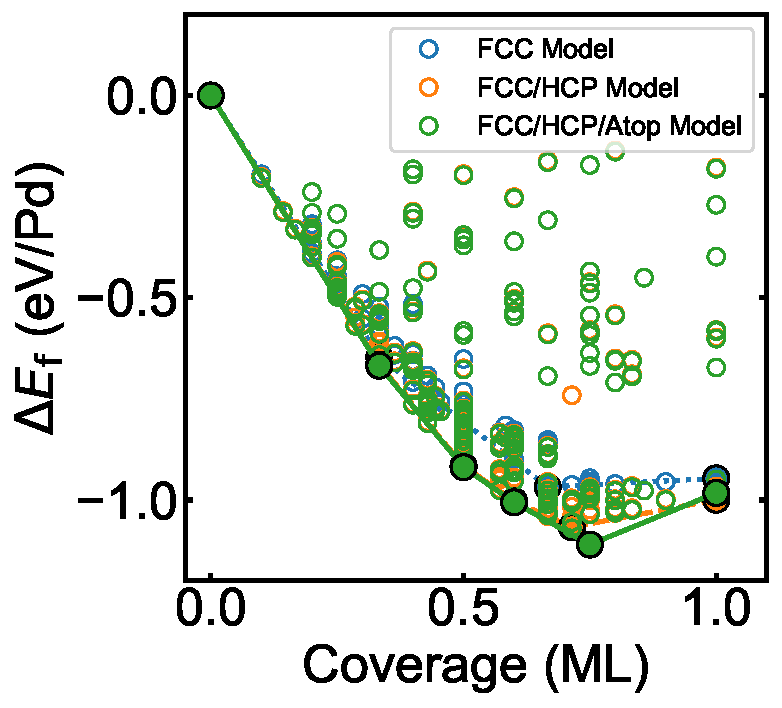
\includegraphics[width=0.8\textwidth]{Figure/FE-com.pdf}
\caption{Comparison of DFT Formation Energies ($\Delta E_\mathrm{f}$) Between the Three Cluster Expansion Models}
\label{DFTcompare}
\end{figure}

\clearpage
\begin{figure} [ht]
\centering
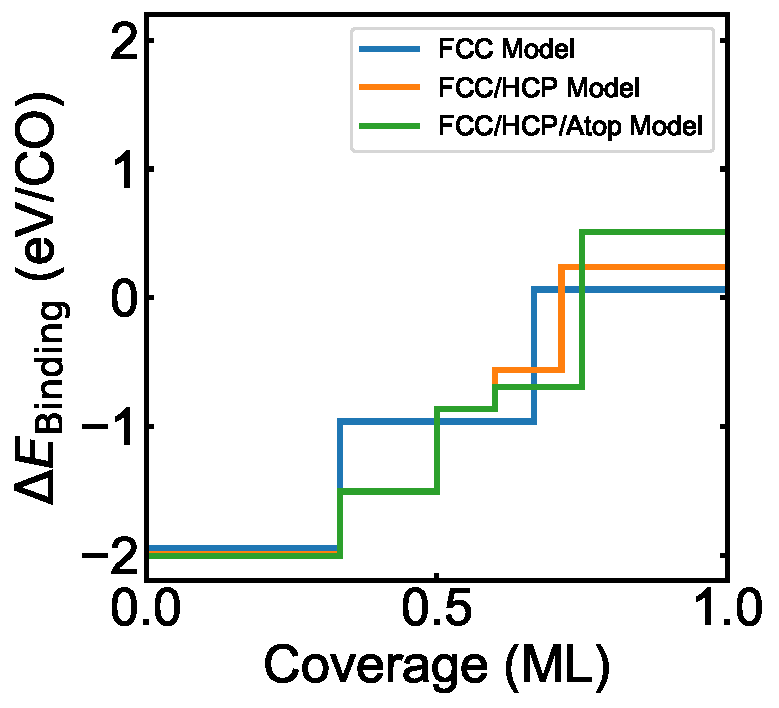
\includegraphics[width=0.8\textwidth]{Figure/BE-com.pdf}
\caption{Comparison of Differential Binding Energy ($\Delta E_\mathrm{Binding}(\theta)$) Between the Three Cluster Expansion Models}
\label{DiffBindingEnergy}
\end{figure}

\end{document}